\chapter{Interpretable Time Series Classification}\label{chapter_sax_vsm}

\section{Introduction}
As I have shown in previous chapters, despite the fact that public software repositories offer a variety of software 
artifacts and accompanying information for scientific research, their intrinsic complexity and the immaturity of 
currently available analysis techniques, which often lack generality, automation, and efficiency, limit the breadth 
and scope of the current MSR research \cite{citeulike:7853299} \cite{citeulike:12550438}.

Addressing this problem, I propose the Software Trajectory Analysis approach -- an automated and efficient technique
for mining of software repositories, that is specifically concerned with the discovery of recurrent behaviors.
This approach is motivated by the evidence that recurrent behaviors are the basic building blocks of software 
processes \cite{neal2012habits} \cite{1903} \cite{citeulike:13208461} and builds upon the hypothesis that it is 
possible to discover recurrent behaviors by the analysis of a specific data type -- ``software trajectories'' -- 
that are sequences of temporally ordered software artifact measurements (i.e., time series constructed of measurements).
While the motivation, background, and evidence leading to this hypothesis were thoroughly discussed in 
previous chapters, here, I introduce a technique that provides the means for its investigation. 
For this, I turn to another research field, which is concerned with the analysis of probably the oldest known 
data type -- the time series \cite{citeulike:1454223} -- and in particular to the research area of 
Time Series Classification (TSC). Since some of the techniques that have been developed and discussed 
within TSC research field are concerned with the unsupervised discovery of class-characteristic features, 
and specifically with the ability to discover \textit{class-characteristic patterns}, which enable the classification, 
the use of such a technique in STA can be effectively translated into the ability to discover class-characteristic 
\textit{meaningful} patterns from software trajectories. 

Later in this Chapter I shall review the current state of the art in TSC, 
propose a novel algorithm for \textit{interpretable} time series classification built upon the discovery of 
class-characteristic patterns, evaluate its performance and the ability to provide an insight into the data and results, 
and discuss the algorithm's use in STA.

\section{Time Series classification}
Time series classification is a well-established and increasingly popular area of research providing solutions to a wide 
range of fields, including, but not limited to data mining, image and motion recognition, environmental sciences, health care, 
and chemometrics. 
Within the last decade, many time series representations, similarity measures, and classification algorithms 
have been proposed following the rapid progress in data collection and storage technologies \cite{citeulike:10358271}. 
Nevertheless, to date, the best overall performing classifier in the field is the one nearest-neighbor algorithm (1NN), 
that can be easily tuned for a particular problem by choosing either a distance measure, an approximation technique, 
or smoothing \cite{citeulike:10358271}.
The 1NN classifier is simple, accurate, robust, depends on a few parameters, and requires no training 
\cite{citeulike:10358271} \cite{citeulike:532340} \cite{citeulike:12563424}.


However, the 1NN technique has a number of significant disadvantages, where the major shortcoming is the 
inability to offer any insight into the classification results. 
Another serious limitation is the need for a significantly large training set representing a within-class 
variance in order to achieve an acceptable accuracy. 
Finally, while having trivial initialization, the nearest neighbor classification is computationally expensive. 
Thus, the demand for an \textit{efficient and interpretable} classification technique capable of processing 
large data volumes remains.

Here, I propose an alternative to 1NN algorithm that addresses the aforementioned limitations. 
In particular, the proposed technique provides a superior interpretability, learns efficiently from a small 
training set, and has a low computational complexity. 

\section{Prior and related work in TSC} \label{sax_vsm_prior}
Almost all of the existing techniques for time series classification can be divided into two major categories \cite{citeulike:11796594}. 
The first category includes techniques based on shape-based similarity metrics where distance is measured directly between 
time series points. A classic example from this category is the nearest-neighbor classifier built upon Euclidean distance 
\cite{citeulike:4214336} or Dynamic Time Warping (DTW) \cite{senin2008dynamic}. 
The second category consists of classification techniques based on structural similarity metrics which employ a high-level 
representation of time series, based on their global and/or local features, for their similarity assessment. 
Examples from this category include classifiers based on a time series representation obtained with 
Discrete Fourier Transform \cite{citeulike:5094223} or Bag-Of-Patterns \cite{citeulike:10525778}. 
The development of these distinct categories can be explained by the significant difference in their performance: 
while shape-based similarity techniques are virtually unbeatable on short pre-processed time series \cite{citeulike:532340}, 
they usually fail on data sets that contain long and noisy time series, 
where structure-based solutions demonstrate the superior performance \cite{citeulike:10525778}. 

Two promising alternatives combining the strengths of techniques from both categories were recently proposed.
The first is the Time Series Shapelet approach that allows for a superior interpretability and delivers a compact 
solution \cite{citeulike:7344347}. 
A shapelet is a short time series ``snippet'' (i.e., subsequence) that is a representative of class membership and is used for 
the decision tree construction facilitating class identification and interpretability.
In order to find the branching shapelet, the algorithm exhaustively searches for the best discriminatory subsequence on data split 
via an information gain measure. The algorithm's classification is built upon the similarity measure between the branching 
shapelet and a full time series, defined as the distance between the shapelet and the closest subsequence in the time series 
when measured by the normalized Euclidean distance. This exact technique, potentially, combines the superior precision of 
exact shape-based similarity methods, and the high-throughput classification capacity of feature-based techniques. 
However, while demonstrating a superior interpretability, robustness, and similar to 1NN algorithm performance, shapelets-based 
technique is computationally expensive, $O(n^{2}m^{3})$, where $n$ is a number of objects and $m$ is the length of a longest 
time series, making its adoption for many-class classification problems difficult \cite{citeulike:11345338}. 
While a better solution was recently proposed ($O(nm^{2})$), it is an approximate approach based on indexing \cite{citeulike:12563493}.

The second technique with interpretable results is the nearest neighbor classifier built upon the Bag-Of-Patterns (BOP) representation of 
time series \cite{citeulike:10525778} which is equated to an Information Retrieval (IR) ``bag of words" concept and is obtained by extraction, 
transformation with Symbolic Aggregate approXimation (SAX) \cite{sax}, and counting the occurrence frequency of short overlapping 
subsequences (i.e., patterns) along the time series.
By applying this procedure to a data set, the algorithm converts it into a vector space, where original time series are 
represented by the pattern occurrence frequency vectors. As the authors has shown, these can be classified with an 1NN classifier 
built with Euclidean distance, or with Cosine similarity that is applied to raw frequencies or their weighted with 
term frequency-inverse document frequency (i.e., \tfidf \cite{salton-71}) values. 
BOP classification has several advantages: its complexity is linear ($O(nm)$), it is rotation-invariant since it accounts for local and 
global structures simultaneously, and it provides an insight into the patterns distribution through frequency histograms.
The authors have concluded that the best classification accuracy of BOP-represented time series is achieved by using 1NN classifier 
based on Euclidean distance. 

\section{SAX-VSM classification algorithm} \label{sax_vsm_background}
I propose the time series classification algorithm called \mbox{SAX-VSM} that extends both aforementioned techniques (i.e., shapelet and BOP). 
In particular, while similar to shapelet-based approaches the algorithm targets the discovery of time series subsequences which 
are the best characteristic representatives of a class, 
instead of the iterative search for a class-discriminating shapelet, \mbox{SAX-VSM} ranks by “importance” all potential candidate 
subsequences \textit{at once} with a \textit{linear computational complexity} of $O(nm)$.
To achieve this, similar to that proposed in BOP, \mbox{SAX-VSM} converts all training time series into bags of SAX 
words and employs \tfidf for their ranking and Cosine similarity for classification. 
Nonetheless, instead of building $n$ bags for each of the training time series, SAX-VSM builds a 
\textit{single bag of words for each of the classes}, which enables effective learning and highly efficient classification ($O(m)$).

As I shall show, these distinct features - the comprehensive summarization of the class' patterns variability with a single bag 
of words and the ranking of each word class-characterization potential - allow SAX-VSM to achieve a high classification accuracy
while providing an exceptional interpretability of the classification results.

\subsection{Preliminaries}
Before describing the algorithm, I shall introduce key terms and concepts used throughout this section, beginning with the data type.
Formally speaking, a time series is an ordered sequence of pairs 
\mbox{$T=((p_{1},t_{1}),(p_{2},t_{2}),...,(p_{i},t_{i}),...,(p_{m},t_{m}))$}
where values $p_{i} \in \mathbf{R^{n}}$ and timestamps are ordered $t_{1} < t_{2} < ... < t_{i} <...<t_{m}$ 
and possibly not equidistant, i.e., $|t_{i}-t_{i-1}| \neq |t_{i}-t_{i+1}|$.

However, in the research literature, without the loss of generality, equispaced data is typically considered implying 
that the raw time series can be treated (i.e., interpolated, aggregated, or approximated) in order to become equispaced. 
Therefore, it is assumed here that the \textbf{\textit{time series}} is a vector of scalar observations: 
$T = ( t_{1},\dots,t_{m} )$, where $t_{i} \in \mathbf{R^{n}}$.

Note, that not-equispaced, irregular data is one of the issues when mining software repositories, as I have discussed previously in 
the Section \ref{section_understanding}, and for this reason STA and SAX-VSM have been designed to effectively mitigate for this: 
STA aggregates raw measurements into software trajectories first, SAX-VSM aggregates and approximates them second. 

In order to rank subsequences by their class-characterization importance, SAX-VSM needs to transform continuous time series data 
into the symbolic (i.e., discrete) representation at first. The algorithm relies on SAX \cite{citeulike:2821475} for discretization and follows 
the best practices of its application. Specifically, it employs the \textit{\textbf{subsequence discretization implemented via a sliding window}}, 
as it is illustrated in the Figure \ref{fig:sliding_window}. By sliding a window along the input time series, SAX-VSM extracts short 
overlapping subsequences and discretizes each of them with SAX. The advantage of this process is that it allows for a better recognition of 
a localized phenomena as it has been shown in the previous research work targeting motifs (recurrent subsequences) \cite{citeulike:3977965} 
and discords (anomalous subsequences) \cite{citeulike:3175749} discovery. 

A time series \textbf{\textit{subsequence}} of length $k$ of a time series $T = (t_{1}, t_{2},...,t_{m})$ of length $m$ is a time 
series $T_{i,k} = (t_{i},t_{i+1},...,t_{i+k-1})$  where $1 \leq i \leq m - k + 1$, i.e., a contiguous fragment of the time series.

\begin{figure}[t]
   \centering
   \includegraphics[width=130mm]{sliding-window.eps}
   \caption[An illustration of the time series symbolic discretization via sliding window.]
   {An illustration of the sliding window technique from \cite{citeulike:2821475}: a time series T of length 128, 
   the subsequence $C_{67}$ (of length $p$=16), and the first 8 overlapping subsequences extracted by a sliding window.}
   \label{fig:sliding_window}
\end{figure}

Subsequence-based SAX discretization requires three parameters to be provided as the input \cite{citeulike:2821475}. 
Currently, to the best of my knowledge, no efficient solution exists for their optimal selection. 
In this work I address this problem by using a cross-validation procedure and a parameters optimization scheme based on the dividing 
rectangles (DIRECT) algorithm that finds optimal parameter values within bounded intervals (i.e., in the range within a minimal and the maximal possible parameter values) \cite{citeulike:12563460}. 
DIRECT is a derivative-free optimization process that possesses local and global optimization properties; converges relatively quickly, and yields a deterministic, optimized solution. While other optimization techniques exist and some of them may perform better, the performance evaluation of the parameters selection scheme is beyond the scope of my current work.

In the following subsections, I shall review all the techniques which are embedded in SAX-VSM. 
Subsection \ref{section-sax} reviews SAX - a symbolic discretization technique, 
Subsection \ref{section_numerosity_reduction} discusses numerosity reduction strategies,
Subsection \ref{bow_representation} reviews bag of words abstraction.
Terms weighting and Vector Space Model are discussed in the Subsection \ref{vsm}. 
SAX-VSM algorithm is presented in the Subsection \ref{sax-vsm}. 


\subsection{Symbolic Aggregate approXimation (SAX)}\label{section-sax}
Discretization of a continuous data into the small number of finite values is highly desirable and often vital for enabling application of machine learning algorithms to datasets reflecting real life phenomena. Hence, probably hundreds of discretization techniques have been developed and are currently available for researchers dealing with knowledge discovery \cite{citeulike:12394286}. Among them, the symbolic representation of time series has attracted much attention by enabling the application of numerous string-processing algorithms, bioinformatics tools, and text mining techniques to continuous data.

One of the most popular algorithms for conversion of time series into symbolic representation is the Symbolic Aggregate approXimation \cite{sax}. 
This technique provides a significant reduction of the time series dimensionality and a lower-bounding to Euclidean distance 
metric, which guarantees no false dismissal \cite{citeulike:2821475}. 
These properties are often leveraged by many time series analysis techniques which exploit SAX in order to increase their efficiency. 
For example, the adoption of SAX indexing allowed for a significantly faster shapelet discovery in \cite{citeulike:12563493}, 
although rendering the algorithm approximate. 

Given a time series $T$ of a length $n$, SAX produces its symbolic approximation $\hat{S}$ of a length $w$ where letters are taken 
from an alphabet $A$. Along with $T$, two parameters must be specified as the input: the alphabet size $\alpha$ and the size of 
the word to produce $w$. The algorithm, whose overview is shown in Figure \ref{fig:sax_intro}, works as follows. 

\begin{figure}[tbp]
   \centering
   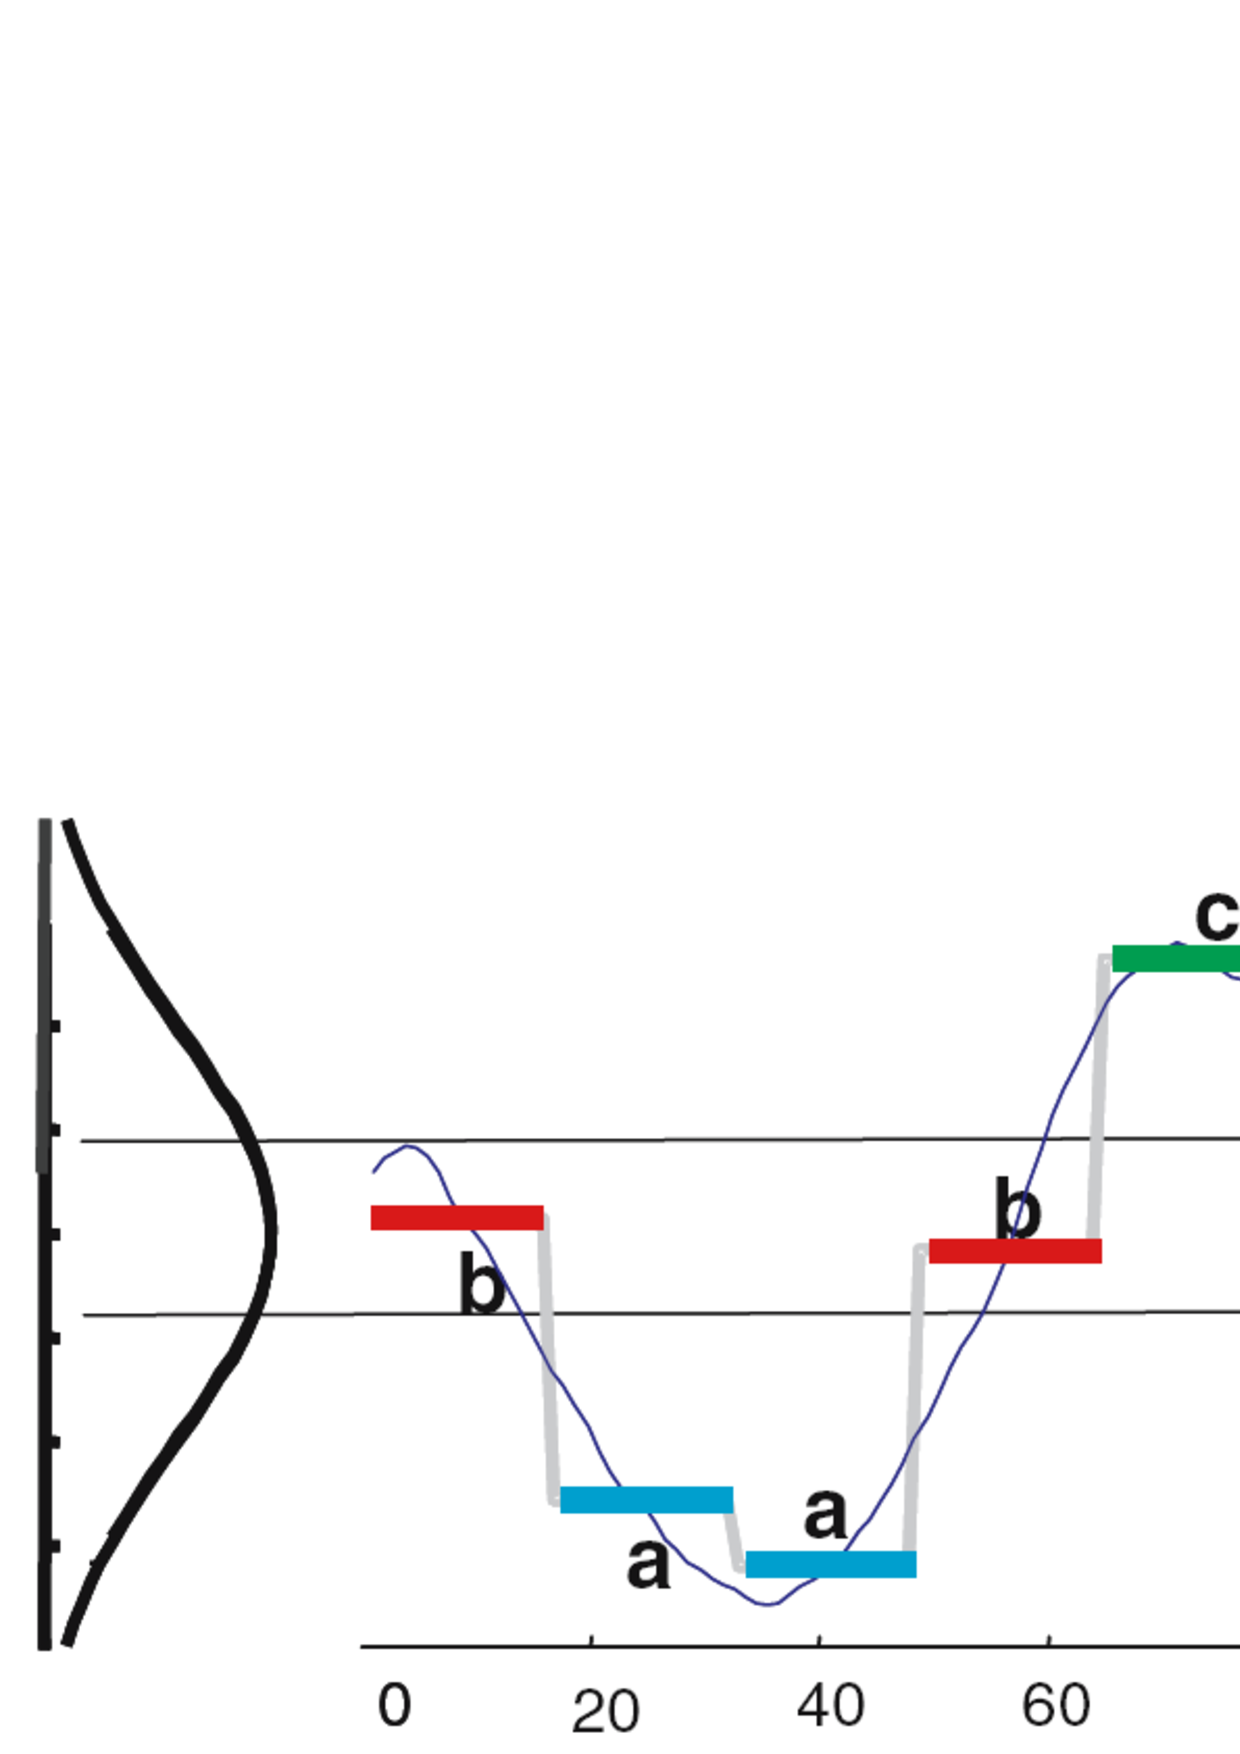
\includegraphics[height=45mm]{sax_intro}
   \caption[An illustration of the Symbolic Aggregate Discretization (SAX) algorithm.]
   {An illustration of the SAX approach taken from \cite{citeulike:2821475} depicts two pre-determined breakpoints for the 
   three-symbols alphabet and the conversion of the time series of length $n=128$ into PAA representation followed by mapping of 
   the PAA coefficients into SAX symbols with $w=8$ and $a=3$ resulting in the string ``\textbf{baabccbc}''.}
   \label{fig:sax_intro}
\end{figure}

At first, since it is meaningless to compare time series with different offsets and amplitudes \cite{citeulike:532340}, the input time 
series $T$ is normalized to unit of standard deviation. This normalization procedure, also known as \textit{z-normalization} or 
``normalization to Zero Mean and Unit of Energy'', allows to minimize the effect of the time series amplitude while preserving time 
series structural specificities \cite{citeulike:3815880}. In order to obtain the normalized time series $\widetilde{T}$, the 
input time series mean is subtracted from each point and the resulting value is divided by their standard deviation:
\begin{equation}
\widetilde{t}_{i} = \frac{t_{i}-\mu}{\sigma}, i \in {1,..,n}
\label{eq:znorm}
\end{equation}
If, however, the standard deviation value falls below a fixed threshold, the normalization procedure is not applied in order to avoid 
a possible over-amplification of the background noise, as it has been shown in \cite{citeulike:2821475}.

At the second step, the dimensionality of the normalized time series is reduced to $w$ by obtaining its 
Piecewise Aggregate Approximation (PAA). For this, $\widetilde{T}$ is transformed into a vector of PAA coefficients $C$ ($|C|=\omega$) 
by dividing it into equal-sized segments and computing their mean values:
\begin{equation}
c_{i} = \frac{w}{n} \sum_{j=\frac{n}{w}(i-1)+1}^{\frac{n}{w}i} \widetilde{t}_{j}
\label{eq:paa}
\end{equation}
Note, that for any $L_{p}$ norm this transformation satisfies to a lower-bounding condition and guarantees no false dismissals
\cite{citeulike:2946589} \cite{citeulike:3000416}.

Discretization is performed at the final step of the SAX algorithm where each of the PAA coefficients obtained at the previous step 
is converted into a letter $\widehat{c}$ of the alphabet $A$ by the use of lookup tables (as shown in Table \ref{sax_table}) 
which define a list of breakpoints 
$B=\beta_{1}, \beta_{2}, ... , \beta_{a-1}$ such that $\beta_{i-1} < \beta_{i}$ and $\beta_{0} = -\infty$, $\beta_{a} = \infty$ 
that divide the area under $N(0,1)$ into $a$ equal areas. 
The design of these tables rests on the assumption that normalized time series tend to have Gaussian distribution \cite{citeulike:10141990} \cite{sax}.
By assigning a corresponding alphabet symbol $\alpha_{j}$ to each interval $[\beta_{j-1},\beta_{j})$, the conversion of the vector of PAA coefficients 
$C$ into the string $\widehat{C}$ implemented as follows: 
\begin{equation}
\widehat{c}_{i} = \alpha_{j}, \; \text{if} \;
{c}_{i} \in [\beta_{j-1},\beta_{j})
\label{eq:sax_alphabet}
\end{equation}

\begin{table}[t]
 \caption[An example of the SAX alphabet breakpoints lookup table.]{An example of the SAX alphabet lookup table that contains the breakpoints dividing a Gaussian distribution in an arbitrary 
number (from 2 to 11) of equiprobable regions.}
 \label{sax_table}
 \small
\begin{tabularx}{\textwidth}{|l|X|X|X|X|X|X|X|X|X|X|}
\hline
\backslashbox{$\beta_{i}$}{$\alpha$} & 2 & 3 & 4 & 5 & 6 & 7 & 8 & 9 & 10 & 11 \\
\hline
$\beta_{1}$ & 0,00 & -0,43 & -0,67 & -0,84 & -0,97 & -1,07 & -1,15 & -1,22 & -1,28 & -1,34  \\
\hline
$\beta_{2}$ &\cellcolor{gray!25}& 0,43 & 0,00 & -0,25 & -0,43 & -0,57 & -0,67 & -0,76 & -0,84 & -0,91  \\
\hline
$\beta_{3}$ &\cellcolor{gray!25}&\cellcolor{gray!25}& 0,67 & 0,25 & 0,00 & -0,18 & -0,32 & -0,43 & -0,52 & -0,60  \\
\hline
$\beta_{4}$ &\cellcolor{gray!25}&\cellcolor{gray!25}&\cellcolor{gray!25}& 0,84 & 0,43 & 0,18 & 0,00 & -0,14 & -0,25 & -0,35 \\
\hline
$\beta_{5}$ &\cellcolor{gray!25}&\cellcolor{gray!25}&\cellcolor{gray!25}&\cellcolor{gray!25}& 0,97 & 0,57 & 0,32 & 0,14 & 0,00 & -0,11  \\
\hline
$\beta_{6}$ &\cellcolor{gray!25}&\cellcolor{gray!25}&\cellcolor{gray!25}&\cellcolor{gray!25}&\cellcolor{gray!25}& 1,07 & 0,67 & 0,43 & 0,25 & 0,11 \\
\hline
$\beta_{7}$ &\cellcolor{gray!25}&\cellcolor{gray!25}&\cellcolor{gray!25}&\cellcolor{gray!25}&\cellcolor{gray!25}&\cellcolor{gray!25}& 1,15 & 0,76 & 0,52 & 0,35  \\ 
\hline
$\beta_{8}$ &\cellcolor{gray!25}&\cellcolor{gray!25}&\cellcolor{gray!25}&\cellcolor{gray!25}&\cellcolor{gray!25}&\cellcolor{gray!25}&\cellcolor{gray!25}& 1,22 & 0,84 & 0,60  \\
\hline
$\beta_{9}$ &\cellcolor{gray!25}&\cellcolor{gray!25}&\cellcolor{gray!25}&\cellcolor{gray!25}&\cellcolor{gray!25}&\cellcolor{gray!25}&\cellcolor{gray!25}&\cellcolor{gray!25}& 1,28 & 0,91  \\
\hline
$\beta_{10}$&\cellcolor{gray!25}&\cellcolor{gray!25}&\cellcolor{gray!25}&\cellcolor{gray!25}&\cellcolor{gray!25}&\cellcolor{gray!25}&\cellcolor{gray!25}&\cellcolor{gray!25}&\cellcolor{gray!25}& 1,34  \\
 \hline
\end{tabularx}
\vspace{0.1cm}
\end{table}

SAX also introduces a new metric for measuring the distance between strings by extending the Euclidean and PAA \cite{citeulike:2946589} distances. 
The function returning the minimal distance between two symbolic representations of the original time series $\widehat{Q}$ and $\widehat{C}$ 
is defined as
\begin{equation}
\text{MINDIST}(\widehat{Q},\widehat{C}) \equiv \sqrt{ \frac{n}{w} } \sqrt{ \sum_{i=1}^{w} ( dist( \widehat{q}_{i}, \widehat{c}_{i} ) )^{2}}
\label{eq:sax_mindist}
\end{equation} 
where the $dist$ function is implemented by using lookup tables specific to a set of used breakpoints (alphabet size) as shown in 
Table \ref{tbl:sax_lookup}, and where the singular value for each cell $(r,c)$ is computed as 
\begin{equation}
cell_{(r,c)} = 
\begin{cases} 
0, \text{ if }\left| r-c \right| \leq 1 \\
\beta_{\max(r,c) - 1} - \beta_{\min(r,c) - 1}, \text{ otherwise}
\end{cases}
\label{eq:cell}
\end{equation}


\begin{table}
\caption[An example of the MINDIST function lookup table.]{An example of the MINDIST function lookup table for the $a=11$}
\label{tbl:sax_lookup}
\small
\begin{tabularx}{\textwidth}{|l|X|X|X|X|X|X|X|X|X|X|X|}
\hline
&\textbf{a}&\textbf{b}&\textbf{c}&\textbf{d}&\textbf{e}&\textbf{f}&\textbf{g}&\textbf{h}&\textbf{i}&\textbf{j}&\textbf{k} \\
\hline
\textbf{a}& 0,00 & 0,00 & 0,43 & 0,73 & 0,99 & 1,22 & 1,45 & 1,68 & 1,94 & 2,24 & 2,67 \\
\hline
\textbf{b}& 0,00 & 0,00 & 0,00 & 0,30 & 0,56 & 0,79 & 1,02 & 1,26 & 1,51 & 1,82 & 2,24 \\
\hline
\textbf{c}& 0,43 & 0,00 & 0,00 & 0,00 & 0,26 & 0,49 & 0,72 & 0,95 & 1,21 & 1,51 & 1,94 \\ 
\hline
\textbf{d}& 0,73 & 0,30 & 0,00 & 0,00 & 0,00 & 0,23 & 0,46 & 0,70 & 0,95 & 1,26 & 1,68 \\ 
\hline
\textbf{e}& 0,99 & 0,56 & 0,26 & 0,00 & 0,00 & 0,00 & 0,23 & 0,46 & 0,72 & 1,02 & 1,45 \\ 
\hline
\textbf{f}& 1,22 & 0,79 & 0,49 & 0,23 & 0,00 & 0,00 & 0,00 & 0,23 & 0,49 & 0,79 & 1,22 \\ 
\hline
\textbf{g}& 1,45 & 1,02 & 0,72 & 0,46 & 0,23 & 0,00 & 0,00 & 0,00 & 0,26 & 0,56 & 0,99 \\ 
\hline
\textbf{h}& 1,68 & 1,26 & 0,95 & 0,70 & 0,46 & 0,23 & 0,00 & 0,00 & 0,00 & 0,30 & 0,73 \\ 
\hline
\textbf{i}& 1,94 & 1,51 & 1,21 & 0,95 & 0,72 & 0,49 & 0,26 & 0,00 & 0,00 & 0,00 & 0,43 \\ 
\hline
\textbf{j}& 2,24 & 1,82 & 1,51 & 1,26 & 1,02 & 0,79 & 0,56 & 0,30 & 0,00 & 0,00 & 0,00 \\ 
\hline
\textbf{k}& 2,67 & 2,24 & 1,94 & 1,68 & 1,45 & 1,22 & 0,99 & 0,73 & 0,43 & 0,00 & 0,00 \\ 
\hline
\end{tabularx}
\end{table}

As shown by Lin et al. \cite{sax}, the SAX distance metric is lower-bounding to the PAA distance, i.e.
\begin{equation}
\sum_{i=1}^{n} (q_{i} - c_{i})^{2} \geq n(\bar{Q} - \bar{C})^{2} \geq n(dist(\hat{Q},\hat{C}))^2
\label{eq:sax_bounding}
\end{equation}

The SAX lower bound was later examined by Ding et al. \cite{citeulike:4501572} and was found to be 
superior in precision to the spectral decomposition methods on non-periodic data sets while only
``slightly'' inferior to other techniques on periodic data. This findings and the capacity of SAX to be
tuned for data specificities made it the best option for symbolic discretization step of SAX-VSM.

%\subsection{SAX discretization of time series}\label{sec_sax_representation}
%One of the ways to represent the time series in symbolic form is to reduce the dimensionality and to 
%discretize the whole time series. The drawback with this approach is that due to the rough approximation 
%it often does not capture enough local details in the data, which severely affects many pattern discovery
%techniques \cite{citeulike:10525778}.  Another way to represent a time series is by a discretization 
%of a collection of overlapping subsequences extracted with a sliding window. 
%
%SAX-VSM relies on this sliding window technique to convert a time series $T$ of a length $m$ into 
%the set of $k$ SAX words, where $k=(m-l_{s})+1$ and $l_{s}$ is the sliding window length. 
%By sliding a window of length $l_{s}$ across time series $T$, extracting subsequences, 
%converting them to SAX words, and placing these words into an unordered collection (a database), 
%it obtains the \textit{bag of words} representation of the original time series $T$.

\subsection{Bag of words representation of time series}\label{bow_representation}
Following its introduction, SAX was shown to be an efficient tool for solving problems 
of finding time series motifs (recurrent patterns) and discords (anomalous patterns) 
in time series \cite{citeulike:3977965, citeulike:3175749}. 
The authors employed a sliding window-based subsequence extraction technique 
and augmented data structures (hash table in \cite{citeulike:3977965} and trie in \cite{citeulike:3175749}) 
in order to index observed SAX words. Further, by analyzing their occurrence frequencies and locations, 
they were able to capture frequent and rare SAX words representing motifs and discords subsequences respectively. 
Later, the same technique based on the combination of sliding window and SAX was used in 
the numerous works, most notably in time series classification using bag of patterns 
(BOP) \cite{citeulike:10525778} and in the Fast-Shapelet algorithm \cite{citeulike:12563493}. 

I also use this sliding window technique to convert a time series $T$ of a length $n$ into 
the set of $m$ SAX words, where $m=(n-l_{s})+1$ and $l_{s}$ is the sliding window length. 
By sliding a window of length $l_{s}$ across time series $T$, extracting subsequences, 
converting them into SAX words, and placing these words into an unordered collection, 
the algorithm builds the \textit{bag of words} representation of the original time series $T$.

\subsection{SAX numerosity reduction}\label{section_numerosity_reduction}
Previously, the analysis of SAX-based algorithms performance by Keogh et al. \cite{citeulike:3977965} and 
Lin et al. \cite{citeulike:3175749} revealed that the best matches for a sliding window 
subsequence tend to be its neighbors, specifically the subsequence one point to the right and the subsequence 
one point to the left -- due to the smoothing effects of PAA approximation and SAX discretization. 
The authors defined these matching subsequences as \textit{trivial matches} and found that in a smooth region 
of a time series the amount of trivial matches can be large enough to dominate over true matches due to 
the over-counting -- an issue which may significantly bias the result and even make it meaningless 
\cite{citeulike:227029} for SAX-based techniques. 
Hence, they have concluded, when extracting subsequences from the time series via a sliding window 
the trivial matches should be excluded. 

The authors proposed a sampling strategy based on a \textit{MINDIST} (Eq. \ref{eq:sax_mindist}) distance 
function designed in order to avoid the trivial and degenerate solutions.
If $l$ consecutive SAX words \newline $\widehat{S}_{i,k}, \widehat{S}_{i+1,k},...,\widehat{S}_{i+l-1,k}$
corresponding to subsequences $T_{i,k}, T_{i+1,k},...,T_{i+l-1,k}$ extracted with sliding window have been
found equal when using \textit{MINDIST}, they kept only the first entry $\widehat{S}_{i,k}$. 
The authors also noted that, similarly to the run length encoding data compression technique, 
if one would ever need to retrieve all the occurrences of $\widehat{S}_{i,k}$, they can be found by sliding 
the window from the first occurrence to the right until the word which is different from $\widehat{S}_{i,k}$ 
is found. 

While the authors found the inclusion of the numerosity reduction vital for motif and discord discovery applications, 
intuitively, since SAX-VSM deals with the classification, an aggressive numerosity reduction may 
in fact reduce the classification performance as it has been shown in the original BOP work \cite{citeulike:10525778}. 
Moreover, by the design of \tfidf statistics (Eq. \ref{formula:tfidf}), the over-counting effect is significantly mediated 
by the inverse document frequency $\text{\textbf{idf}}$ that efficiently reduces the effect of high word counts 
proportionally to their inter-class occurrence.

In order to clarify this issue, I have conducted an exploratory study of the SAX numerosity reduction 
effect on SAX-VSM performance. In a series of experiments, I have found, that for most of used data sets, the application of 
numerosity reduction significantly reduces the DIRECT scheme convergence time and, sometimes, improves the classification accuracy. 
Furthermore, once I have relaxed the trivial match constraints by the substitution of 
\textit{MINDIST} with a distance function based on the Hamming distance \cite{hamming}, 
I was able to slightly improve the classification accuracy for more than half of the data sets used for \mbox{SAX-VSM}
performance evaluation as shown in the Table \ref{perf_table2} (SAX-VSM accuracy results obtained with the ``exact'' 
value of numerosity reduction parameter). 
The \textit{HAMMING} distance function for two SAX words $\hat{Q}$ and $\hat{C}$ of the same length $w$ 
is defined as the count of letters in which they differ:
\begin{equation}
\label{eq:hamming}
\begin{split}
\text{HAMMING}(\widehat{Q},\widehat{C}) \equiv \sum_{i=1}^{w} I( \widehat{q}_{i}, \widehat{c}_{i} ), \\
\text{where } I( \widehat{q}_{i}, \widehat{c}_{i} ) = 
\begin{cases}
 1,\text{ if } \widehat{q}_{i} \neq \widehat{c}_{i} \\
 0,\text{ if } \widehat{q}_{i} = \widehat{c}_{i}
\end{cases}
\end{split}                                                      
\end{equation}

For further use, I abbreviate the numerosity reduction strategy based on the previous work (i.e., on \textit{MINDIST} 
function) as \textit{\textbf{CLASSIC}}, while the one based on \textit{HAMMING} distance as \textit{\textbf{EXACT}}.

Note that, as the experimental evaluation has shown, the effect of the numerosity reduction strategy may or may not be significant 
for a particular dataset, moreover, since this effect is impossible to know in advance, the numerosity reduction strategy becomes 
yet another parameter which needs to be properly selected in order to achieve the best SAX-VSM performance for a given dataset. 
Therefore, in total, there are four parameters which need to be optimized for the SAX-VSM application to a particular dataset.

\subsection{Vector Space Model (VSM) adaptation}\label{vsm}
I use the Vector Space Model exactly as it is known in Information Retrieval (IR) \cite{citeulike:300428} for 
manipulations with abstracted by SAX words time series subsequences. 

Similarly to IR, I define and use the following expressions:
\begin{itemize}
  \item \textit{term} - a single SAX word;
  \item \textit{bag of words} - an unordered collection of SAX words, i.e., terms;
  \item \textit{corpus} - a set of bags;
  \item \textit{term frequency matrix} - a matrix defining the term occurrence frequency for each bag, 
  whose rows correspond to all observed in a corpus terms and whose columns correspond to bags;
  \item \textit{term weight matrix} - a similar to term frequency matrix structure defining the weight coefficient 
  of a term for each of the corpus' bags;
  \item document (bag) \textit{term weight vector} - a column of the weight matrix defining weights of all terms for a single bag.
\end{itemize}
Note however, that I use terms \textit{bag of words} and \textit{document} for abbreviation of an unordered 
collection of SAX words interchangeably, while in IR these usually bear different meaning as a \textit{document} 
presumes words ordering (i.e., semantics). 
Although similar definitions, such as \textit{bag of features} \cite{citeulike:12636726} 
or \textit{bag of patterns} \cite{citeulike:10525778}, were recently proposed for techniques built 
upon SAX \cite{citeulike:10525778}, I use the traditional \textit{bag of words} definition since it reflects 
my workflow best. 

Given a training set of time series, that is typically built from labeled sets of time series (i.e., ``classes''), 
SAX-VSM builds a single bag of SAX words for each of the classes by processing all class' time series with a sliding 
window and SAX. Then, these bags are combined into a corpus 
which in turn is transformed into the term frequency matrix, whose rows correspond to the set of all SAX words (terms) 
found in \textit{all classes}, whereas each column denotes a class of the training set. 
Each element of this matrix is an observed frequency of a term in a class. 
Note, that because SAX words extracted from time series of one class are often not among other classes, 
as it is shown further in the Section \ref{scalability}, this matrix is usually sparse. 
%Many elements of this matrix are zeros - because words extracted from one class 
%are often not found in others (Figure \ref{fig:venn}). 
%By its design, this sparse term frequency matrix is a dictionary of all SAX words extracted from all time 
%series of a training set, which accounts for frequencies of each word in each of 
%the training classes.

\begin{table}
\caption{The SMART notation. }
\vspace{0.4cm}
\label{tbl:smart}
{\footnotesize
\begin{tabularx}{\textwidth}{l l l}
\toprule[1pt]
\textbf{Term frequency} &\textbf{Document frequency} &\textbf{Normalization} \\[0.5ex]
\midrule
\textbf{n} (natural):  $\text{tf}_{t,d}$ & \textbf{n} (no): 1 & \textbf{n} (none): 1 \\[2ex]
\textbf{l} (logarithm): $1+log(\text{tf}_{t,d}$) & \textbf{t} (idf): $log\tfrac{N}{df_{t}}$ & \textbf{c} (cosine): $\tfrac{1}{\sqrt{w_1^2 + w_2^2 + ... + w_M^2}}$ \\[2ex]
\textbf{a} (augmented): $0.5 + \tfrac{0.5 \times \text{tf}_{t,d}}{\text{max(tf}_{t,d})}$ & \textbf{p} (prob idf): $\textbf{max}\left( 0,\text{log}\tfrac{N-df_{t}}{df_{t}} \right) $ & 
\textbf{b} (byte size): $\tfrac{1}{CharLength^\alpha}, \alpha < 1 $ \\[2ex]
\textbf{b} (boolean): $\begin{cases} 1, & \text{if tf}_{t,d} > 0 \\ 0, & \text{otherwise} \end{cases} $ & & \\[3ex]
\textbf{L} (log average): $ \tfrac{1+\text{log}(\text{tf}_{t,d})}{1+\text{log}(\text{ave}_{t \epsilon d}( \text{tf}_{t,d}))}$ & & \\[1ex]
\bottomrule[1pt]
\end{tabularx}
}
\end{table}

Following to the common in IR workflow, SAX-VSM employs the \tfidf weighting scheme \cite{citeulike:4469058} for each element 
of this matrix in order to transform the frequency value into a weight coefficient. 
The \tfidf weight for a term is defined as a product of two factors: term frequency ($\text{\textbf{tf}}$) 
and inverse document frequency ($\text{\textbf{idf}}$). 
For the first factor, I use logarithmically scaled term frequency (Table \ref{tbl:smart}) \cite{citeulike:4469058}:
\begin{equation}
 \mbox{\textbf{tf}}_{t, d} =  \begin{cases} 1 + \log(\mbox{\textbf{f}}_{t,d}), &\mbox{if \textbf{f}}_{t,d}>0  \\
0, & \mbox{otherwise} \end{cases}
\end{equation} 
where $t$ is a term and $d$ is a bag of words (the document in IR terms), and $\mbox{\textbf{f}}_{t,d}$ 
is a frequency of the term in the bag.
For the second factor I use inverse document frequency:
\begin{equation}
 \mbox{\textbf{idf}}_{t, D} =  \log_{10}\frac{|D|}{|d \in D : t \in d|} = \log_{10}\frac{N}{\mbox{\textbf{df}}_{t}}
 \label{formula:idf}
\end{equation} 
where $N$ is the cardinality of corpus $D$ (the total number of bags) and the 
denominator $\mbox{\textbf{df}}_{t}$ is a number of bags where the term $t$ appears.

Thus, the \tfidf value for a term $\textit{t}$ in the document 
$\textit{d}$ of a corpus $\textit{D}$ is defined as:
\begin{equation}
 \text{\textbf{tf}} \ast \text{\textbf{idf}}(t, d, D) =  \text{\textbf{tf}}_{t, d} \times \text{\textbf{idf}}_{t, D} = \log(1 + \text{\textbf{f}}_{t,d})
\times \log_{10}\frac{N}{\mbox{\textbf{df}}_{t}}
 \label{formula:tfidf}
\end{equation} 
for all cases where $\mbox{\textbf{f}}_{t,d}>0$ and $\mbox{\textbf{df}}_{t}>0$, or zero otherwise.
Once all terms of a corpus are weighted, the term frequency matrix becomes a term weight matrix and its columns 
are used as the class' \textit{term weight vectors} that facilitate the classification with Cosine similarity. 

The Cosine similarity measure between two vectors is defined by their inner product and magnitude. 
For two vectors $\mathbf{a}$ and $\mathbf{b}$ that is:
\begin{equation}
%\mbox{similarity}(\boldsymbol{a},\boldsymbol{b}) = cos(\theta) = \frac{ \sum\limits^{n}_{i=1} a_{i}
%\times b_{i} }{
%\sqrt{\sum\limits^{n}_{i=1} a_{i}} \times \sqrt{\sum\limits^{n}_{i=1} b_{i}} }
\mbox{similarity}(\mathbf{a},\mathbf{b}) = cos(\theta) = 
\frac{ \mathbf{a} \cdot \mathbf{b} } {\left| \left| a \right| \right| \cdot \left| \left| b \right|\right|} =
\frac{ \sum\limits_{i=1}^{n}{a_{i} \times b_{i}} }{ \sqrt{\sum\limits_{i=1}^{n}{(a_{i})^2}} \times \sqrt{\sum\limits_{i=1}^{n}{(b_{i})^2}}}
\label{eq:cosine_similarity}
\end{equation} 

\subsection{SAX-VSM implementation} \label{sax-vsm}
As many other time series structure-based classification techniques, SAX-VSM consists of two 
phases - the training (i.e., learning of class-characteristic patterns) and the classification. 
Within the training phase, SAX-VSM discretizes all labeled time series with SAX and builds $N$ bags 
of SAX words, where $N$ is the number of classes. 
Then, by applying the \tfidf weighting scheme to the corpus of $N$ bags it obtains $N$ weight vectors 
which it uses for the time series classification procedure built upon the Cosine similarity. 
The schematic overview of the algorithm training and classification phases is given in the Figure \ref{fig:sax-vsm_overview}.

\begin{figure}[t]
   \centering
   \includegraphics[width=148mm]{figures/SAX-VSM_overview.eps}
   \caption[An overview of the SAX-VSM algorithm.]{
   An overview of the SAX-VSM algorithm: 
   at first, labeled time series are converted into bags of words using SAX; 
   secondly, $\text{\textbf{tf}}\ast\text{\textbf{idf}}$ statistics is computed resulting in 
   a single weight vector per training class. For the classification, an unlabeled 
   time series is converted into the term frequency vector and assigned a 
   label of the weight vector that yields a maximal cosine similarity value.
   This is \textit{\textbf{ltc.nnn}} weighting schema in SMART notation (Table \ref{tbl:smart}).}
   \label{fig:sax-vsm_overview}
\end{figure}

\subsubsection{Training}
SAX-VSM training starts by the transformation of all labeled time series into SAX representation. 
This process is configured by four parameters: 
the sliding window length (\textit{W}), 
the number of PAA segments per window (\textit{P}), 
SAX alphabet size (\textit{A}),
and the numerosity reduction strategy.
Note that each subsequence extracted with a sliding window is normalized (Sec. \ref{section-sax}) 
before being processed with PAA, however, if the standard deviation value falls below a fixed threshold, 
the normalization is not applied in order to avoid over-amplification of the background noise \cite{sax}. 

By applying this procedure to all time series from $N$ training classes, the algorithm builds a corpus of 
$N$ word bags. 
Then, it computes weights of all of the corpus' terms using \tfidf and outputs $N$ real-valued weight vectors of 
equal length representing training classes. 

Because the whole training set must be processed, training of SAX-VSM classifier is computationally 
expensive ($O(nm)$, where $n$ is the number of time series and $m$ is the maximal length of the time series). 
However, there is no need to maintain an index of training time series, or to keep any 
of them in the memory at runtime -- the algorithm simply iterates over all training time series building 
bags of SAX words incrementally. Once built and weighted with \tfidf, the corpus is discarded -- only the
resulting set of $N$ real-valued weight vectors is retained for the classification.

\subsubsection{Classification}
In order to classify an unlabeled input time series, SAX-VSM transforms it into a terms frequency vector using 
exactly the same sliding window technique and SAX parameters set that were used for the training. 
Then, it computes cosine similarity values between this vector and $N$ \tfidf weight vectors that represent 
training classes. The input time series is assigned to the class whose vector yields the maximal cosine 
similarity value.

\begin{figure}[t]
   \centering
   \includegraphics[width=150mm]{figures/figure_direct.eps}
   \caption[An illustration of the DIRECT-driven SAX-VSM parameters optimization for \textit{SyntheticControl} dataset.]
   {An illustration of the DIRECT-driven SAX-VSM parameters optimization for \textit{SyntheticControl} dataset. 
   The left panel shows all points sampled by DIRECT in the space \mbox{$PAA*Window*Alphabet$}.
   The red points correspond to high error values while green points correspond to low error values 
   in cross-validation experiments. 
   Note the green points concentration at $W$=42. 
   Middle panel shows the classification error heat map obtained by a complete scan 
   of all 432 points of the hypercube slice when $W$=42. 
   Right panel shows the classification error heat map of the same slice when 
   the parameters search was optimized by DIRECT, 
   the optimal solution ($P$=8,$A$=4) was found by sampling just 43 points.}
   \label{fig:direct-sampling}
\end{figure}

\section{Parameters optimization} \label{section-direct}
As shown above, in total, SAX-VSM requires four discretization parameters to be specified upfront from which three 
(the sliding window length, the PAA size, and the SAX alphabet size) may vary in a wide range. 
Unfortunately, to the best of my knowledge, there is no efficient solution known for their selection.

Addressing this issue I propose a solution based on a common cross-validation and \mbox{DIRECT} \mbox{(DIviding RECTangles)} 
optimization scheme \cite{citeulike:4210208}. As I shall show, the combination of these techniques allows for 
an optimal parameter selection while using only the training data. For brevity, I omit the detailed explanation 
of the DIRECT algorithm background and motivation, referring the interested reader to the original work 
\cite{citeulike:12563460} for additional details.

DIRECT is designed to deal with a parameters optimization problems of form:
\begin{equation}
 \min_{x} \: f(x), \: f \in \mathbf{R}, \: x, X_{L}, X_{U} \in \mathbf{R}, \: \text{where} \: X_{L} \leq x \leq X_{U}
 \label{formula:direct}
\end{equation} 
where $f(x)$ is the error function, and $x$ is the parameters vector.
At the first step DIRECT scales the search domain to the unit hypercube. The function is then evaluated 
at the center point of the hypercube. As pointed in \cite{citeulike:12563460}, computing the function value
at the center is an advantage of the method when dealing with problems
in higher dimensions.
Then, DIRECT iteratively performs two procedures - partitioning the hypercube into smaller hyper-rectangles 
and identifying a set of potentially-optimal ones by sampling their centers. At each step, the function is evaluated 
at the center points of all potentially-optimal hyper-rectangles. The procedure continues interactively until the 
error function converges. Note, that DIRECT is guaranteed to converge to the global optimal function value,
as the number of iterations approaches to infinity \cite{citeulike:12563460}.

\begin{figure}[!t]
   \centering
   \includegraphics[width=145mm]{beef_thesis_direct_plot.ps}
   \caption[An illustration of the numerosity reduction strategy effect on parameters optimization process.]
   {An illustration of the numerosity reduction strategy effect on DIRECT-driven parameters optimization process. 
   The points represent the error rate in cross-validation experiments and are colored according to its value: 
   the red color indicates high error values, while the green corresponds to low error values. 
   Note that dense points collocations are differ among strategies, which indicates the difference in their error 
   function gradient.
   }
   \label{fig:sax_nr}
\end{figure}

Since DIRECT is designed to search for global minima of a real valued function over a bound constrained domain, 
whereas SAX parameters are natural numbers, I employ the rounding of a reported solution values to the nearest integer.
Figure \ref{fig:direct-sampling} illustrates the application of leave-one-out cross-validation and DIRECT to the
\textit{SyntheticControl} data set \cite{ucr} which consists of 6 classes. 
In this case, the algorithm converged after sampling just 130 out of 13,860 possible parameters combinations -- 
that is over 100x speedup.

Figure \ref{fig:sax_nr} shows the effect of each of the numerosity reduction strategies on parameters optimization
process with DIRECT for Beef dataset that features time series classes obtained by measuring a degree of beef contamination 
by adulterants with mid-infrared spectroscopy \cite{citeulike:12859637}. 
Sixteen iterations of DIRECT were performed for each experiment. 
The optimal solution (Window=19, PAA=17, Alphabet=3) was found with \textit{EXACT} numerosity reduction strategy 
in 8 iterations; without numerosity reduction, optimization process converged in 10 iterations, while 
with \mbox{\textit{MINDIST}-based} numerosity reduction in 9 iterations. 
Note the differences in sampled locations between strategies: without numerosity reduction, DIRECT efficiently found 
the minima location after sampling of 317 locations, whether with reduction, a number of close to optimal locations was 
found earlier and thus sampled more rigorously. 
365 locations were sampled with \mbox{\textit{MINDIST}-based} numerosity reduction, and 369 locations with Hamming-based 
numerosity reduction, which indicates an increase in the optimization process sensitivity when a numerosity reduction is used.

Note, that the parameters optimization scheme discussed above does not include the numerosity reduction strategy.
The reasons for this is that the numerosity reduction strategy mostly affects the parameters optimization scheme 
convergence speed rather than the accuracy of the classification, thus, for the most cases, it can be simply pre-defined 
to \textit{EXACT}.
%Secondly, since the numerosity reduction procedure is applied after the discretization, it is possible to branch the 
%code execution at that point and to compute 

\section{Intuition behind SAX-VSM}
First, by combining \textit{\textbf{all}} SAX words extracted from 
\textit{\textbf{all}} time series of single class into a \textit{\textbf{single bag}} of 
words, SAX-VSM manages to effectively capture and summarize the observed intraclass variability 
even from a small training set.  

Second, by normalizing, smoothing, approximating time series subsequences, and discarding their 
original ordering, SAX-VSM focuses exclusively on the local structural phenomena regardless of the 
data distortion by the rotation and its corruption by the noise or values loss.

Third,  \tfidf statistics naturally highlights terms that are unique to the class by assigning them high weights, 
whereas terms that observed in multiple classes are assigned low, 
inversely proportional to their interclass presence, weights. 
This improves the selectivity of the classification by decreasing the contribution of ``confusive'' multi-class terms, 
while increasing the contribution of unique ``class-defining'' terms to the final similarity measurement value.

Ultimately, the algorithm compares the set of subsequences extracted from an unlabeled time series 
with the weighted set of all characteristic subsequences representing the whole of the training class. 
Thus, an unknown time series is classified by its similarity not to a given number of 
``neighbors'' as in kNN or BOP classifiers, or to a single characteristic subsequence, as in shapelet-based classifier, 
but by the \textit{combined similarity} of all its subsequences to all known discriminative patterns found in the 
whole of the class.

\begin{table}[t]
\caption{Description of the datasets used in performance evaluation.}
\vspace{0.4cm}
 \label{data_typetable1}
\centering
{\setlength{\extrarowheight}{2pt}%
{\footnotesize
\begin{tabularx}{\linewidth}{@{} l l @{}}
\hline
Class type Dataset & Datasets \\[0.5ex]
\hline
Image data & 50 words, Adiac, Yoga , Face Four, Face all, Faces UCR, Fish, \\
 & Swedish Leaf, OSU Leaf, Arrow Head, Shield, Diatom, Medical Images \\[0.5ex]
Motion data & Gun-Point, Cricket, Cricket-NEW, Sony AIBO walk, Pass Graph, \\ 
 & uWaveGesture \\[0.5ex]
Spectroscopy data & Beef, Coffee, Olive Oil, Wheat \\[0.5ex]
Synthetic datasets & Cylinder-Bell-Funnel, Synthetic Control, Two Patterns, Mallat \\[0.5ex]
Energy consumption & Italy Power Demand, Electrical Devices \\[0.5ex]
Medical measurements & ECG200, ECG 5 days, Medical images, ECG Thorax \\[0.5ex]
Other measurements obtained with instruments & Trace, Lightning 2, Lightning 7, Wafer, Ford A, Ford B, \\
 & Chlorine concentration, Starlight \\[0.5ex]
\hline
\end{tabularx}
}}
\end{table}

\section{SAX-VSM performance evaluation} \label{results}
I have proposed a novel algorithm for time series classification based on SAX approximation of time series and 
Vector Space Model called SAX-VSM. In this section I describe a set of experiments assessing its performance and 
exploring its ability to provide an insight into the classification results.

\subsection{Analysis of the classification accuracy}
I have evaluated SAX-VSM accuracy on 45 datasets, whose majority was taken from the benchmark data disseminated 
through the UCR repository \cite{ucr}. These datasets represent a variety of data types that reflect typical TSC 
domain problems. Table \ref{data_typetable1} describes their origin.

Table \ref{perf_table1} compares the classification accuracy of \mbox{SAX-VSM} with 
previously published results for four competing classifiers: 
two state-of-the-art 1NN classifiers based on Euclidean distance and DTW, 
and two interpretable classifiers based on recently proposed Fast-Shapelets technique \cite{citeulike:12563493} 
and BOP \cite{citeulike:10525778} on 19 datasets.
I have selected these particular techniques in order to position \mbox{SAX-VSM} in terms of 
the classification accuracy and the results interpretability. 

\begin{table}[t!]
\captionsetup{justification=centering}
\caption{Classification accuracy comparison for state of the art nearest-neighbor, interpretable, and \mbox{SAX-VSM} classifiers.}
 \label{perf_table1}
{\setlength{\extrarowheight}{1.5pt}%
{\footnotesize
\begin{tabularx}{\linewidth}{@{} l *6X @{}}
\hline
Dataset & \mbox{Num. of} classes & 1NN-Euclidean & 1NN-DTW & Fast Shapelets &  \mbox{Bag Of} \mbox{Patterns}
& SAX-VSM\\
\hline
Adiac        &37  & 0.389   & 0.391  & 0.514  & 0.432  & \textbf{0.381}\\
Beef         &5   & 0.467   & 0.467  & 0.447  & 0.433 & \textbf{0.3}\\
CBF         & 3  & 0.148    & 0.003  & 0.053    & 0.013 & \textbf{0.002} \\
Coffee       &2    & 0.250   & 0.180  & 0.067     & 0.036     & \textbf{0.0} \\
ECG200     &2   & \textbf{0.120}  & 0.230  & 0.227     & 0.140   & 0.140 \\
FaceAll      &14  & 0.286   & \textbf{0.192}  & 0.402     & 0.219   & 0.207\\
FaceFour    &4   & 0.216   & 0.170  & 0.089     & 0.011   & \textbf{0.0} \\
Fish         &7   & 0.217   & 0.167  & 0.197    & 0.074   & \textbf{0.017} \\
Gun-Point    &2   & 0.087   & 0.093  & 0.060     & 0.027     & \textbf{0.007} \\
Lightning2    &2   & 0.246   & \textbf{0.131}  & 0.295  & 0.164  & 0.196 \\
Lightning7    &7   & 0.425   & \textbf{0.274}  & 0.403  & 0.466  & 0.301 \\
Olive Oil     &4   & \textbf{0.133}   & \textbf{0.133}  & 0.213     & \textbf{0.133}  & \textbf{0.133}\\
OSU Leaf    &6   & 0.483   & 0.409  & 0.359     & 0.236  & \textbf{0.107} \\
Syn.Control  &6   & 0.120   & \textbf{0.007}  & 0.081     & 0.037  & 0.010 \\
Swed.Leaf   &15  & 0.213   & 0.210 & 0.270 & \textbf{0.198} & 0.251 \\
Trace       &4   & 0.240   & \textbf{0.0}    & 0.002  & \textbf{0.0} & \textbf{0.0} \\
Two patterns &4   & 0.090   & \textbf{0.0}    & 0.113   & 0.129      & 0.006 \\
Wafer        &2    & 0.005   & 0.020     & 0.004  & 0.003 & \textbf{0.0006} \\
Yoga        &2    & 0.170   & \textbf{0.164}  & 0.249 & 0.170 & \textbf{0.164} \\
\hline
\end{tabularx}
}}
\end{table}

Table \ref{perf_table2} compares the classification accuracy of SAX-VSM with 
1NN state of the art classifiers based on Euclidean and DTW distances on all 45 datasets. 
Fast-Shapelet and BOP classifiers were excluded from this comparison table because their 
performance for these datasets is unknown.

\clearpage

\begin{table}[t!]
\caption{Classification accuracy comparison for state of the art nearest-neighbor and SAX-VSM classifiers.}
 \label{perf_table2}
\centering
{\setlength{\extrarowheight}{1pt}%
{\scriptsize
\begin{tabularx}{\linewidth}{@{} l *7X @{} l}
%\begin{tabularx}{\linewidth}{l c c c c c c c l}
\hline
Dataset & \mbox{Num. of} classes & Training set size & Testing set size & Series length & 1NN-Euclidean & 1NN-DTW & SAX-VSM & Discretization param. \\
\hline
Synthetic Control & 6 & 300 & 300 & 60 & 0.12 & \textbf{0.007} & 0.0133 & 45,7,5,exact \\
CBF & 3 & 30 & 900 & 128 & 0.148 & 0.003 & \textbf{0.0021} & 55,4,12,nored \\
Gun Point & 2 & 50 & 150 & 150 & 0.087 & 0.093 & \textbf{0.066} & 32,12,9,exact \\
50 words & 50 & 450 & 455 & 270 & 0.369 & \textbf{0.310} & 0.3582 & 190,10,3,exact \\ 
Trace & 4 & 100 & 100 & 275 & 0.24 & \textbf{0.0} & \textbf{0.0000} & 220,16,11,exact \\
Adiac & 37 & 390 & 391 & 176 & 0.389 & 0.396 & \textbf{0.3810} & 100,24,16,nored \\
Yoga & 2 & 300 & 3000 & 426 & 0.170 & \textbf{0.164} & \textbf{0.1639} & 70,14,15,nored \\ 
Beef & 5 & 30 & 30 & 470 & 0.467 & 0.5 & \textbf{0.3} & 19,17,3,exact \\ 
Coffee & 2 & 28 & 28 & 286 & 0.25 & 0.179 & \textbf{0.0} & 107,22,3,nored \\
Olive Oil & 4 & 30 & 30 & 570 & \textbf{0.133} & \textbf{0.133} & \textbf{0.1330} & 460,52,13,classic \\
ECG200 & 2 & 100 & 100 & 96 & \textbf{0.12} & 0.23 & 0.1400 & 44,9,5,exact \\
ECG 5 days & 2 & 23 & 861 & 136 & 0.065 & 0.232 & \textbf{0.0100} & 41,11,4,exact \\
Face all & 14 & 560 & 1,69 & 131 & 0.286 & \textbf{0.192} & 0.2065 & 42,8,4,nored \\
Face four & 4 & 24 & 88 & 350 & 0.216 & 0.170 & \textbf{0.1112} & 67,7,5,exact \\
Fish & 7 & 175 & 175 & 463 & 0.217 & 0.167 & \textbf{0.0171} & 99,19,8,nored \\
Swedish Leaf & 15 & 500 & 625 & 128 & 0.213 & \textbf{0.210} & 0.2512 & 49,9,7,exact \\
OSU Leaf & 6 & 200 & 242 & 427 & 0.483 & 0.409 & \textbf{0.0867} & 33,8,12,nored \\
Lightning 2 & 2 & 60 & 61 & 637 & 0.246 & 0.131 & \textbf{0.1967} & 169,15,3,nored \\
Lightning 7 & 7 & 70 & 73 & 319 & 0.425 & 0.274 & \textbf{0.3287} & 97,17,3,nored \\
Wafer & 2 & 1 & 6,174 & 152 & 0.005 & 0.020 & \textbf{0.0010} & 34,32,7,classic \\
Two Patterns & 4 & 1 & 4 & 128 & 0.09 & \textbf{0.0} & 0.0040 & 107,12,3,nored \\
Ford A & 2 & 3,601 & 1,32 & 500 & 0.3182 & 0.484 & \textbf{0.1272} & 80,10,5,exact \\
Ford B & 2 & 3,636 & 810 & 500 & 0.4086 & 0.495062 & \textbf{0.2567} & 80,10,5,exact \\
Chlorine Concentration & 3 & 467 & 3840 & 166 & 0.35 & 0.352 & \textbf{0.3341} & 30,27,5,classic \\
Cricket & 2 & 9 & 98 & 166 & 0.0511 & \textbf{0.0102} & \textbf{0.0102} & 165,10,4,exact \\
Cricket - NEW & 2 & 9 & 98 & 166 & 0.4375 & \textbf{0.125} & 0.2343 & 165,10,4,exact \\
Sony AIBO walk & 2 & 20 & 601 & 70 & 0.3045 & 0.2745 & \textbf{0.2628} & 54,4,16,exact \\
PassGraph & 2 & 69 & 131 & 364 & 0.3664 & 0.2824 & \textbf{0.2812} & 119,10,15,nored \\
Wheat Spectrography & 7 & 49 & 726 & 1050 & 0.44 & 0.457 & \textbf{0.2790} & 130,50,10,nored \\
Arrowhead & 3 & 36 & 175 & 625 & 0.32 & 0.32 & \textbf{0.3028} & 113,11,3,classic \\
Shield & 3 & 30 & 129 & 1179 & 0.1395 & 0.1395 & \textbf{0.0772} & 150,12,4,nored \\
Mallat & 8 & 320 & 2080 & 256 & \textbf{0.0235} & 0.0312 & 0.0274 & 214,10,15,nored \\ 
uWaveGesture\_X & 8 & 896 & 3582 & 315 & \textbf{0.2607} & 0.2725 & 0.2635 & 260,7,5,exact \\
uWaveGesture\_Y & 8 & 896 & 3582 & 315 & \textbf{0.3384} & 0.3659 & 0.3534 & 240,10,4,exact \\
uWaveGesture\_Z & 8 & 896 & 3582 & 315 & 0.3504 & 0.3417 & \textbf{0.3400} & 258,8,4,exact \\
Diatom Size Reduction & 4 & 16 & 306 & 345 & 0.0654 & \textbf{0.0327} & 0.0653 & 174,15,18,exact \\
Medical Images & 10 & 381 & 760 & 99 & 0.3158 & \textbf{0.2631} & 0.4802 & 29,9,5,exact \\
Words Synonyms & 25 & 267 & 638 & 270 & 0.3824 & \textbf{0.3511} & 0.4404 & 198,10,3,exact \\
FacesUCR & 14 & 200 & 2050 & 131 & 0.2307 & 0.0951 & \textbf{0.0751} & 38,8,3,exact \\
Symbols & 6 & 25 & 995 & 398 & 0.1005 & \textbf{0.0503} & 0.1015 & 112,12,5,exact \\
Starlight Curves & 3 & 1000 & 8236 & 1024 & \textbf{0.0632} & 0.093 & 0.0807 & 172,15,11,exact \\
Italy Power Demand & 2 & 67 & 1029 & 24 & 0.0949 & \textbf{0.0495} & 0.1166 & 13,16,5,exact \\
ElectricalDevices & 7 & 8953 & 7745 & 96 & 0.9132 & 0.9132 & \textbf{0.3227} & 17,13,6,nored \\
ECG Thorax1 & 42 & 1800 & 1965 & 750 & 0.171 & \textbf{0.209} & 0.2340 & 44,15,14,exact \\
ECG Thorax2 & 42 & 1800 & 1965 & 750 & 0.120 & \textbf{0.135} & 0.1450 & 44,15,14,exact \\
\hline
\end{tabularx}
}}
\end{table}

\clearpage
Note, that in the evaluation, I followed the train/test data split as provided by UCR. 
At first, the train data was used in the cross-validation for optimization of SAX parameters 
using \mbox{DIRECT}. Second, once found, the optimal parameter settings were used to assess SAX-VSM 
classification accuracy on the test data. 
The last column of table Tables \ref{perf_table1} and \ref{perf_table2} reports the SAX-VSM 
classification accuracy and the parameter settings.

\subsection{Scalability analysis} \label{scalability}
For synthetic data sets, it is possible to create as many instances as one needs for the experimentation. 
Moreover, the ground truth corresponding to their features and patterns is always known through their design.
I have used Cylinder-Bell-Funnel \cite{cbf} and Two Patterns \cite{two_patterns} synthetic datasets 
in order to investigate and to compare the performance of SAX-VSM and 1NN Euclidean classifier on increasingly 
large data sets.

\begin{figure}[t]
   \centering
   \includegraphics[width=140mm]{figures/cbf.ps}
   \caption{An example of the three classes from CBF dataset.}
   \label{fig:cbf}
   %\vspace{1cm}
   %\includegraphics[width=140mm]{figures/funnels.ps}
   %\caption{An example of a variation in Funnel class.}
   %\label{fig:funnel}
\end{figure}

\subsubsection{Cylinder-Bell-Funnel (CBF) dataset}
The CBF problem was introduced in \cite{cbf} and since then has been routinely used in TSC for the investigation 
of a classifier performance behavior.
The dataset represents a classical problem of time series classification where the class assignment is made upon the 
detection of a \textit{single global} pattern. 
The goal is to separate three classes of objects: cylinder ($c$), bell ($b$), and funnel ($f$).  Figure \ref{fig:cbf} 
shows examples of time series from each of the classes. 
The Cylinder is characterized by a plateau, the Bell by an increasing linear ramp followed by a sharp drop, 
while the Funnel is characterized by a sharp rise followed by a gradual decrease. 
The class-characteristic feature start, its duration (length of the plateau and ramps) and the amplitude are randomized. 
Gaussian noise is also added to each time series point:

\noindent\begin{minipage}{.5\linewidth}
\begin{equation*}
\begin{split}
 &c(t)=(6+\eta)\cdot\chi_{[a,b]}(t)+\epsilon(t) \\
 & b(t)=(6+\eta)\cdot\chi_{[a,b]}(t)\cdot(t-a)/(b-a)+\epsilon(t) \\
 & f(t)=(6+\eta)\cdot\chi_{[a,b]}(t)\cdot(b-t)/(b-a)+\epsilon(t)
\end{split}
\end{equation*}
\end{minipage}%
\begin{minipage}{.5\linewidth}
\begin{equation}
\label{eq:cbf}
\text{, where }
\chi_{[a,b]}=\begin{cases}
0,t < a \\
1,a\leq t\leq b\\
0,t > b \end{cases}
\end{equation}
\end{minipage}

\noindent where $\eta$ and $\epsilon(t)$ are drawn from a standard normal distribution $N(0,1)$, $a$ is an integer 
drawn uniformly from the interval $[16,32]$ and $(b-a)$ is drawn uniformly from $[32,96]$.

\subsubsection{Two patterns dataset}
As mentioned, the CBF problem demands a classifier to make the decision based on a single global pattern. 
Contrary, the Two Patterns problem requires a classifier to recognize ordered occurrences of two local patterns.

In particular, patterns that are used to define classes are the upward step and the downward step,
as it is shown in Figure \ref{fig:2patterns}. Class $DD$ corresponds to two downward steps, $DU$ to the succession
of a downward and an upward step, etc. The position and the duration of these patterns are randomized, 
which creates an additional challenge for a classifier to distinguish classes with similar patterns, i.e., $UD$ and $DU$.
The signal surrounding patterns is randomized with the Gaussian noise. 
As pointed by the dataset author, this problem is particularly challenging for classical learning 
algorithms that do not account for the sequential measurements dependency \cite{two_patterns}.

\begin{figure}[t]
   \centering
   \includegraphics[width=140mm]{figures/2patterns.ps}
   \caption{An example of the four classes from Two Patterns dataset.}
   \label{fig:2patterns}
\end{figure}

\subsection{Classification scalability}
In a series of experiments, I varied the training data set size from $5$ to $1,600$ instances of each time series class, 
while the test data set size remained fixed to $10,000$ instances. 
For small training sets, SAX-VSM was found to be significantly more accurate than 1NN classifier based on Euclidean 
distance but less accurate than 1NN classifier based on DTW. 
However, by the time there were more than $400$ time series in a training set, there was no statistically 
significant difference in accuracy between all classifiers, 
as shown at left panels of Figures \ref{fig:precision-runtime} and \ref{fig:2p-precision-runtime}. 

\begin{figure}[t]
   \centering
   \includegraphics[width=140mm]{figures/cbf-precision-runtime.ps}
   \caption[Classification accuracy and run time comparison for SAX-VSM and 1NN classifiers on CBF data.]
   {Classification accuracy and run time comparison for SAX-VSM and 1NN classifiers on CBF data.
   SAX-VSM performs significantly better than 1NN Euclidean classifier with 
   a limited amount of training samples, but not as good as 1NN DTW classifier (left panel). 
   While SAX-VSM is fastest in the classification, its performance is comparable to 1NN Euclidean classifier 
   when the training time is accounted for (right panel).}
   \label{fig:precision-runtime}

   \includegraphics[width=140mm]{figures/2patterns-precision-runtime.ps}
   \caption[Classification accuracy and run time comparison for SAX-VSM and 1NN classifiers on Two Patterns data.]
   {Classification accuracy and run time comparison for SAX-VSM and 1NN classifiers on Two Patterns data.
   Experiment reveals that on small training set sizes the problem is much harder 
   for SAX-VSM and 1NN Euclidean classifiers than it is for the 1NN DTW classifier. 
   Nevertheless, similarly to the previous experiment, SAX-VSM performs better than 1NN Euclidean classifier
   in terms of the both: accuracy and speed.}
   \label{fig:2p-precision-runtime}
\end{figure}

As per the running time cost, to no surprise, the DTW-based classifier was found to be the most expensive technique. 
Due to the comprehensive training, SAX-VSM was found to be more expensive than 1NN Euclidean 
classifier on small training sets, but outperformed it on larger training sets.

However, SAX-VSM can perform the training offline and can load class-characteristic \tfidf weight vectors when needed. 
If this option can be utilized, the proposed classifier performs significantly faster than both 1NN classifiers as 
shown at the right panels of Figures \ref{fig:precision-runtime} and \ref{fig:2p-precision-runtime}.

\begin{figure}[t]
   \centering
   \includegraphics[width=140mm]{figures/words-cbf.ps}
   \caption[An illustration of the SAX-VSM class-characteristic pattern vectors size evolution for the CBF dataset 
   with increasingly large training set size.]{An illustration of the SAX-VSM class-characteristic pattern vectors
   size evolution for the CBF dataset 
   with increasingly large training set size (left panel), and the distribution of terms in the CBF corpus for 
   a training set of one million time series of each class.}
   \label{fig:venn-cbf}

   \includegraphics[width=140mm]{figures/words-two-patterns.ps}
   \caption[An illustration of the SAX-VSM class-characteristic pattern vectors size evolution for the Two Patterns dataset 
   with increasingly large training set size.]{An illustration of the SAX-VSM class-characteristic pattern vectors size evolution for the Two Patterns dataset 
   with increasingly large training set size (left panel), and the distribution of terms in the Two Patterns corpus for 
   a training set of one million time series of each class.}
   \label{fig:venn-2p}
\end{figure}

\subsubsection{SAX-VSM training scalability}
In another series of experiments I have investigated the scalability of the algorithm with
unrealistic training set sizes - up to one million of instances of each of CBF classes.
As expected, with the growth of the training set size, the curve for a total number of distinct SAX
words and curves for dictionary sizes of each of CBF classes reflected a significant saturation 
as it is shown at the left panel of Figure \ref{fig:venn-cbf}. 
For the largest of training sets - $10^6$ instances of each class - the size of the dictionary peaked at $67,324$ 
of distinct words (which is less than 10\% of all possible words of length 7 from an alphabet of 7 letters), 
and the largest \tfidf vector accounted for $23,569$ values (Figure \ref{fig:venn-cbf}, right). 
In my opinion, this result reflects two characteristics of the data set chosen: the first is that the diversity of words which 
are possible to encounter in CBF dataset is quite limited by its classes configuration (i.e., single global 
pattern) and by the choice of SAX parameters (smoothing). 
The second specificity is that IDF (Inverse Document Frequency, \ref{formula:idf})
efficiently limits the growth of dictionaries by eliminating those words, which are observed in all
classes. 

The similar behavior was observed in the experimentation with Two Patterns dataset. 
The Figure \ref{fig:venn-2p} shows the rapid saturation of SAX word dictionaries as a training dataset grows in size.


\subsection{Robustness to noise}\label{saxvsm_robustness}
As shown, the growth of the dimensionality of \tfidf weight vectors follows the growth of the training set size, which indicates that SAX-VSM is continuously learning from the observed class variability. Since the weight of each of overlapping subsequences extracted from time series via sliding window contributes only a small fraction to the final similarity value, and since each subsequence represents a localized structural phenomenon, intuitively, the SAX-VSM classifier shall be robust to the noise and to the partial signal loss. In this case, the cosine similarity between two high dimensional weight vectors may not degrade significantly enough to cause misclassification (Equation \ref{eq:cosine_similarity}).

\begin{figure}[t]
  \centering
  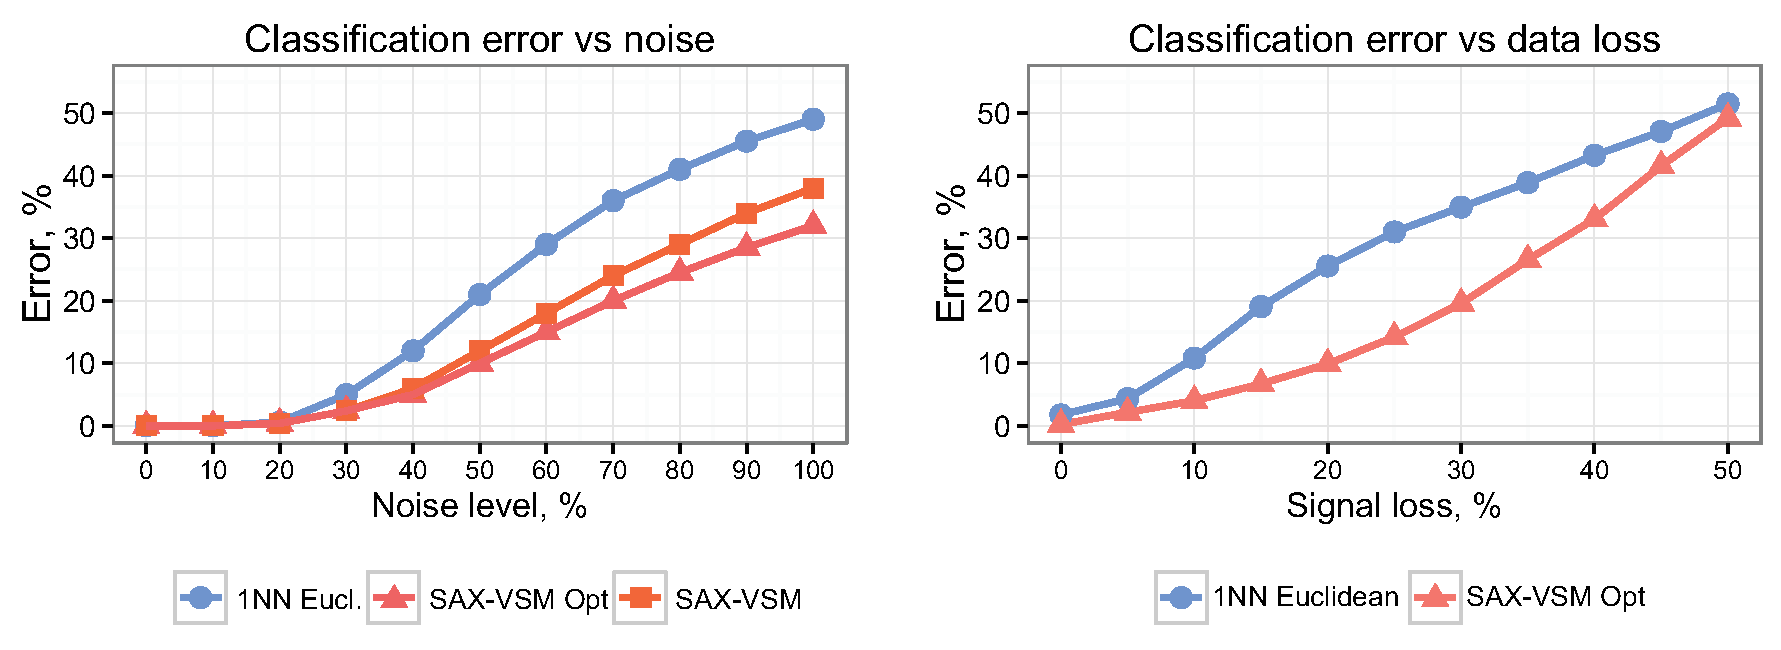
\includegraphics[width=130mm]{figures/corrupted.eps}
  \caption[An illustration of the SAX-VSM classification performance evolution on CBF dataset with added noise and signal loss.]
  {An illustration of the SAX-VSM classification performance evolution on CBF dataset with added noise 
  (left panel, the random noise amplitude varies up to 100\% of that of the signal value),
  and with a signal loss 
  (right panel, the start and stop of the``lost interval'' were chosen randomly).
  \textit{SAX-VSM Opt} curves correspond to the results obtained with the ``optimized'' for each case 
  SAX parameters.}
  \label{fig:corrupted}
\end{figure}

In one series of experiments, by fixing a training set size to 250 time series, I have varied the standard deviation 
of Gaussian noise in CBF model (whose default value is about 17\% of a signal level). 
I have found, that SAX-VSM increasingly outperformed 1NN Euclidean classifier with the growth of the noise level 
(Fig.\ref{fig:corrupted} Left). 
Further improvement of SAX-VSM performance was achieved by the tuning of the PAA smoothing through a gradual 
increase of the sliding window size proportionally to the growth of the noise level 
(Fig.\ref{fig:corrupted} Left, \textit{SAX-VSM Opt} curve). 

In another series of experiments, I replaced up to 50\% of an unlabeled time series span with a randomly placed 
stretches of the Gaussian noise, mimicking the signal corruption. 
Again, SAX-VSM performed consistently better than 1NN Euclidean classifier regardless of the training set size, 
which I have varied from 5 to 1'000. 
The \textit{SAX-VSM Opt} curve at Fig.\ref{fig:corrupted} (Right) depicts an experiment where the training set size
was fixed to 50 time series of each class and when the sliding window size was decreased inversely proportionally 
to the signal loss growth.

\subsection{Interpretable classification}
While the classification performance results in previous sections confirms that SAX-VSM 
classifier has a comparable to state of the art classification performance, 
its major strength is in the level of allowed interpretability of classification results. 

Previously, in the original shapelets work \cite{citeulike:7344347, citeulike:11957982}, it has been shown 
that the resulting decision tree offers an insight into the data specificity through class-characteristic patterns.
In the successive work based on shapelets \cite{citeulike:11345338}, it was also shown that the 
discovery of multiple shapelets provides increasingly better resolution and intuition into the interpretability 
of classification. 

However, as the authors noted, the runtime cost of multiple shapelets discovery in a many class problems 
can be prohibitive to the approach applicability. In contrast, SAX-VSM extracts and weights all patterns at once, 
without any added cost. Therefore, it could be the only choice for interpretable classification in many class problems.

Further in this section, I propose a SAX-VSM based heatmap-like time series class specificity visualization 
that provides insight into the classification result and show the utility of the subsequence ranking for 
interpreting of the class-characteristic data specificity.

\begin{figure}[!h]
   \centering
   \includegraphics[width=130mm]{figures/cbf-heatmap.ps}
   \caption[An example of the heatmap-like visualization that exploits SAX-VSM subsequence ranking in order to 
   highlight time series segments that are highly characteristic to the class.]{An example of the heatmap-like visualization that exploits SAX-VSM subsequence ranking in order to 
   highlight time series segments that are highly characteristic to the class.
   Highlighted by the visualization features corresponding to a sudden rise, plateau, and a sudden drop in Cylinder, 
   increasing trend in Bell,
   and to a sudden rise followed by a gradual drop in Funnel, 
   align exactly with the design of these classes \cite{cbf}.}
   \label{fig:heat1}
   \includegraphics[width=130mm]{figures/2patterns-heatmap.ps}
   \caption[An example of the heatmap-like visualization for Two Patterns dataset.]{An example of the heatmap-like visualization for Two Patterns dataset, which also confirms the proposed 
   algorithm's ability to capture the class specificity in more challenging than CBF settings where class-characteristic 
   patterns are local and ordered \cite{two_patterns}.}
   \label{fig:heat2}
\end{figure}

\subsubsection{Heatmap-like visualization}
Since SAX-VSM builds \tfidf weight vectors using all subsequences extracted from a
training set, it is possible to find out the weight of any arbitrary selected subsequence.
This feature enables a novel visualization technique that can be used to gain an immediate
insight into the layout of ``important'' class-characterizing subsequences as it is shown in Figures
\ref{fig:heat1} and \ref{fig:heat2}.

In order to highlight class-characteristic subsequences, the color hue value for each point is computed as the combination of 
\tfidf weights of all subsequences that span the point. If the subsequence is found to be characteristic to other than the 
analyzed time series class, its weight is subtracted, if it belongs to the same class, the weight is added. 

This type of visual analysis allows for an immediate insight into the classification results as for any of the classified 
time series it is possible to visualize which subsequences were found class-characteristic for each of the classes and to 
which degree.

\subsubsection{Gun Point data set}
By following the previously mentioned shapelet-based work \cite{citeulike:7344347} \cite{citeulike:11345338}, 
I have used a well-studied \textit{\mbox{Gun/Point}} data set \cite{Ratanamahatana04makingtime-series} to explore the 
interpretability of classification results. This data set contains two classes: 
time series in the \textit{Gun} class corresponds to the actor's hand motion when drawing
a replicate gun from a hip-mounted holster, pointing it at the target for a second, and returning the gun to the holster; 
time series in the \textit{Point} class corresponds to the actor's hand motion when pretending
of drawing a gun --- the actor points her index finger to a target for about a second, and then returns the 
hand to her side. 

\begin{figure}[t]
   \centering
   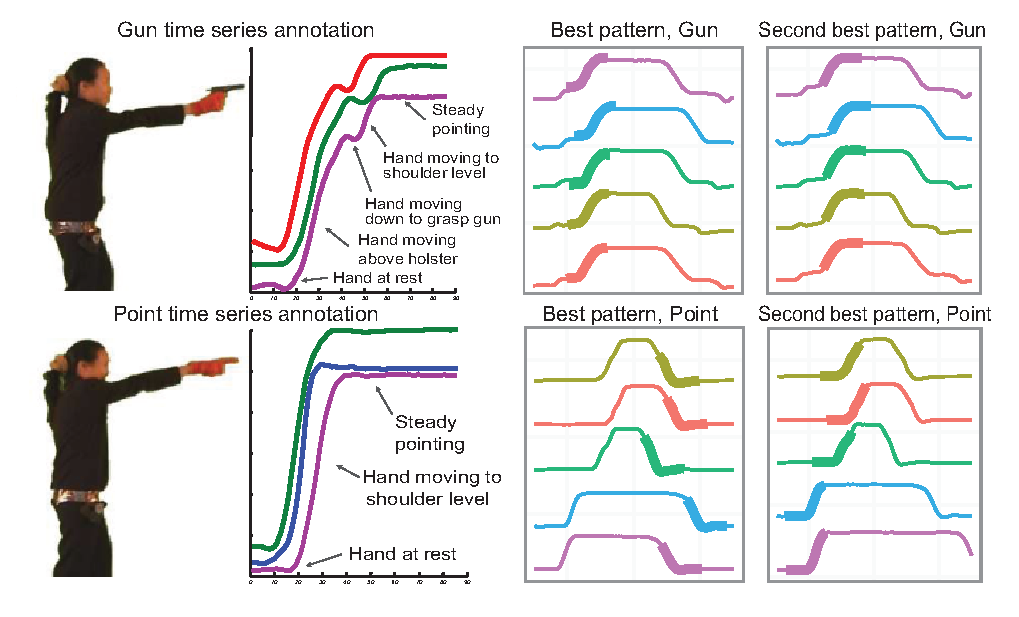
\includegraphics[width=130mm]{figures/gun-point.eps}
   \caption[Best class-characteristic subsequences (right panels, bold lines) discovered by SAX-VSM in
   the \textit{Gun/Point} data set.]{Best class-characteristic subsequences (right panels, bold lines) discovered by SAX-VSM in
   the \textit{Gun/Point} data set. 
   Left panels show actor's stills and the time series annotation made by an expert while the right panels 
   show locations of characteristic subsequences.
   Note, that while the upward arm motion found to be more ``important'' in the \textit{Gun} class 
   (gun retrieval and aiming), the downward arm motion better characterizes the \textit{Point} class 
   (note the ``overshoot'' phenomena in propless arm return). 
   This result aligns with previous work \cite{citeulike:7344347} and \cite{citeulike:11345338}.
   (Stills and annotation are used with a permission from E. Keogh) }
   \label{fig:shapelet-like-patterns}
\end{figure}

Similarly to previously reported results \cite{citeulike:7344347} \cite{citeulike:11345338}, 
SAX-VSM captured all distinguishing features as shown in Figure \ref{fig:shapelet-like-patterns}. 
The most weighted by SAX-VSM pattern in \textit{Gun} class corresponds to fine extra movements required to 
lift and aim the prop. 
The most weighted pattern in \textit{Point} class corresponds to the ``overshoot'' phenomena that is causing the 
characteristic dip in the time series. 
Also, similarly to the original \textit{GunPoint} work \cite{Ratanamahatana04makingtime-series}, as second to the best 
pattern in \textit{Point} class, SAX-VSM highlighted the lack of distinguishing subtle extra movements required
for lifting a hand above the holster and reaching down for the gun.

\begin{figure}[!h]
   \centering
   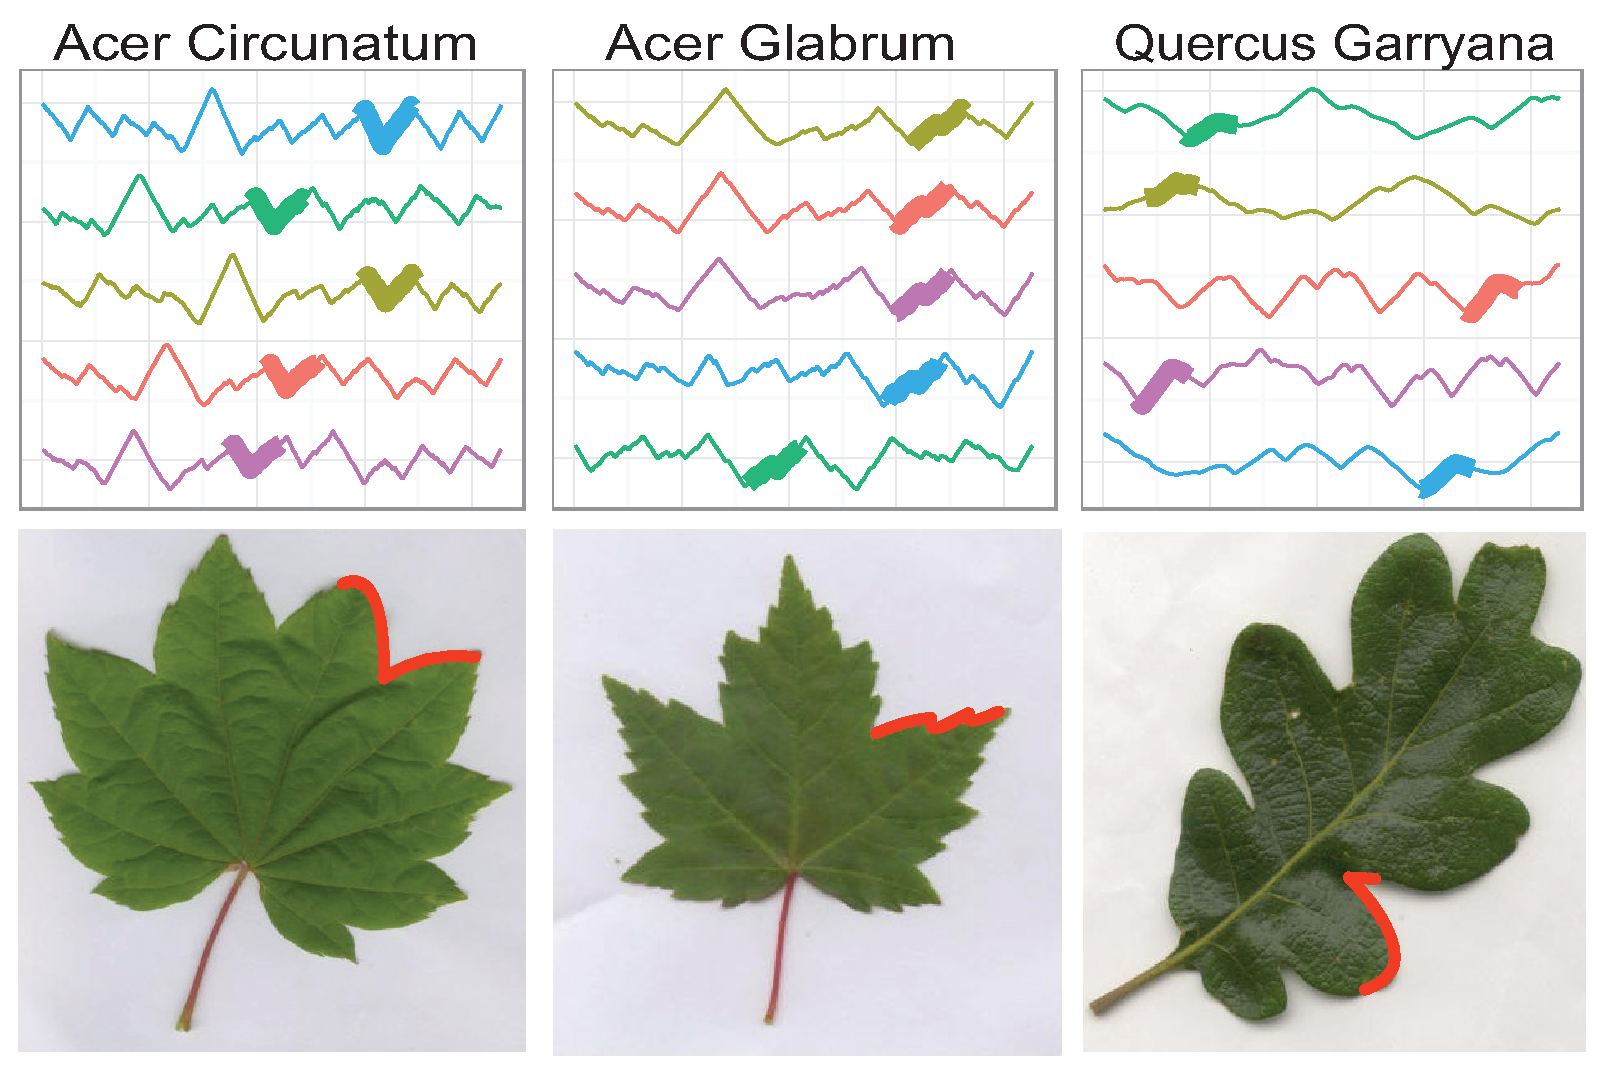
\includegraphics[width=130mm]{figures/AcerCircunatum.eps}
   \caption[The best class-characteristic subsequences (top panels, bold lines) discovered by SAX-VSM in
    the \textit{OSULeaf dataset}.]{The best class-characteristic subsequences (top panels, bold lines) discovered by SAX-VSM in
    the \textit{OSULeaf dataset}. These patterns align exactly with well known in botany leaves discrimination techniques
    by the lobe shape, serration, and tip type \cite{citeulike:12134192}.}
   \label{fig:shapelet-acer-patterns}
\end{figure}

\subsubsection{OSU Leaf data set}
According to the original data source, A.Grandhi \cite{citeulike:12563798}, with the growth of digitized data 
volumes, there is a huge demand for automatic management and retrieval of various images. 
The \textit{OSULeaf} data set consist of curves obtained by image segmentation and boundary
extraction (in the anti-clockwise direction) from digitized leaf images of six classes: \textit{Acer Circinatum, 
Acer Glabrum, Acer Macrophyllum, Acer Negundo, Quercus Garryana} and \textit{Quercus Kelloggii}.
The authors of the original work were able to solve the problem of leaf curve classification by using 
the nearest neighbor classifier built upon DTW distance achieving 61\% of the classification accuracy. 

Since SAX-VSM performed significantly better on this problem, I have investigated the classification results.
In contrast to NN classification results that do not offer any insights, SAX-VSM application yielded a set of 
class-specific characteristic patterns for each of six classes of leaves from \textit{OSULeaf} data set. 
Further patterns investigation revealed, that they closely match known techniques for leaves classification based 
on their shape and margin \cite{citeulike:12134192}. 
Highlighted by SAX-VSM features include 
the slightly lobed shape and acute tips of Acer Circinatum leaves, 
the serrated blade of Acer Glabrum leaves, 
the acuminate tip and a characteristic serration of Acer Macrophyllum leaves, 
the pinnately compound leaves arrangement of Acer Negundo, 
the incised leaf margin of Quercus Kelloggii, 
and the lobed leaf structure of Quercus Garryana. 
Figure \ref{fig:shapelet-acer-patterns} shows a subset of these characteristic patterns and the original
leaf images with highlighted features that correspond to SAX-VSM discovered patterns.

\begin{figure}[!h!t]
   \centering
   \includegraphics[width=120mm]{figures/coffee_patterns.ps}
   \caption[The best class-characteristic subsequences (left panels, bold lines) discovered by SAX-VSM in
   the \textit{Coffee data set}.]{The best class-characteristic subsequences (left panels, bold lines) discovered by SAX-VSM in
   the \textit{Coffee data set}. Right panels show zoom-in view on these subsequences in Arabica
   and Robusta spectrograms.
   These discriminative subsequences correspond to the chlorogenic acid (best subsequence) 
   and to the caffeine (second to best) regions of spectra. This result aligns with
   the ground truth and the original work based on PCA \cite{citeulike:12550833} exactly.  }
   \label{fig:coffee}
\end{figure}

\subsubsection{Coffee data set}
Another illustration of interpretable classification with SAX-VSM is based on the Coffee dataset \cite{citeulike:12550833}.
The time series for this problem were obtained with the Fourier transform infrared spectroscopy instrument equipped 
with a diffuse reflection sampling station (DRIFT). The raw time series were truncated to 286 data points which represent 
the observed spectra within the 800-1900 cm$^{-1}$ range. 

The two top-ranked by SAX-VSM subsequences in both datasets correspond to spectrogram intervals accounting for
abundances of Chlorogenic acid (the best characteristic pattern) and Caffeine (the second to best characteristic pattern).
These two chemical compounds are known to be responsible for the flavor differences in Arabica and Robusta coffees; 
moreover, these spectrogram intervals were also reported as discriminative when used in the PCA-based classification 
technique developed by the authors of the original work \cite{citeulike:12550833}.

\subsubsection{Characteristic pattern utility}
As shown above, via discovered by SAX-VSM class-characteristic patterns we can learn the inherent structure of the analyzed data in a manner that allows intuitive interpretation of classification results. In addition, ranked class-characteristic pattern vectors provide a compact way to summarize data classes. 

Note, that in contrast to shapelet-based techniques, which are based on the single class-characteristic pattern, SAX-VSM generates a ranked list of patterns, which, once computed, allows much deeper insight into the studied phenomena through the examination of  second best, third, and so on, patterns. 
When compared with BOP approach, where a list of ranked patterns is built for each class' entity, SAX-VSM, which aggregates patterns into a single bag, provides a naturally better way to summarize the class-characteristic specificity. 

\section{Clustering}\label{saxvsm_clustering}
Clustering is a generic technique used for data partitioning, visualization, and exploration.
In addition, clustering is an important subroutine in many data mining algorithms \cite{citeulike:167581}.
Since clustering algorithms are built upon a distance function, that computes similarity between clustered entities,
the algorithm's performance is highly dependent on the performance of the chosen distance function. 
Thus, an experimental evaluation of the proposed in this chapter technique in clustering shall provide an additional 
perspective on its performance and the applicability beyond the classification.

\subsection{Hierarchical clustering}
Probably, one of the most used clustering algorithms is hierarchical clustering which requires no
parameters to be specified as input \cite{citeulike:1576606}. It computes pairwise distances between all objects 
and produces a nested hierarchy of clusters offering the efficient data partitioning and visualization. 

Previously, it has been shown that the bag-of-patterns time series representation along with the Euclidean distance
provide superior clustering performance\cite{citeulike:10525778}. 
For comparison, I have performed a similar experiment that only differ in the time series representation and
the distance metric -- I have used \tfidf weight vectors obtained from SAX-VSM and the Cosine similarity. 
Confirming previous work, I have found, that the combination of SAX and Vector space model outperforms 
classical shape-based distance metrics. 
For example, Figure \ref{fig:hc} depicts the result of a hierarchical clustering of the data subset from 
\textit{SyntheticControl} dataset. 
Obviously, the data partitioning obtained with SAX-VSM clustering is superior those based on Euclidean and DTW 
distance metrics as it properly splits data into three valid branches.

\begin{figure}[!h!t]
   \centering
   \includegraphics[width=120mm]{figures/clustering.eps}
   \caption[A comparison of the distance metrics performance in hierarchical clustering for the subset of three
   \textit{SyntheticControl} classes: \textit{Normal, Decreasing trend}, and \textit{Upward shift}.]
   {A comparison of the distance metrics performance in hierarchical clustering for the subset of three
   \textit{SyntheticControl} classes: \textit{Normal, Decreasing trend}, and \textit{Upward shift}. 
   The Euclidean distance and Dynamic Time Warping were applied to raw time series while the Cosine similarity 
   was applied to their representation as term weights vectors. Complete linkage was used to generate clusters. 
   Only SAX-VSM was able to partition the data properly.   }
   \label{fig:hc}
\end{figure}

\subsection{k-Means clustering}
Another popular choice for data partitioning is k-Means clustering algorithm \cite{kmeans}.
The basic intuition behind this algorithm is that through the iterative reassignment of objects 
into different clusters the intra-cluster distance is minimized. 

As it has been shown before, k-Means algorithm scales much better than hierarchical partitioning techniques 
\cite{citeulike:4195343}. In addition, k-Means clustering is also well studied in IR field. 
For example in \cite{citeulike:505248}, the authors extensively examined seven different criterion functions for 
partitional document clustering and found, that \textit{k}-prototypes partitioning with cosine dissimilarity 
(the approach similar to \mbox{SAX-VSM}) delivers an excellent performance. 

Following this work, I have implemented a similar to \cite{citeulike:1172599} \textit{spherical k-means algorithm}
and found, that it converges quickly and delivers a satisfactory partitioning on short synthetic data sets. 
Further, I have evaluated the technique on the long time series from PhysioNet archive \cite{citeulike:699487}, 
from which I have extracted 250 time series corresponding to five vital signals: 
two ECG leads (aVR and II), RESP, PLETH, and CO2 waves, trimming them to 2'048 points. 
Similarly to BOP experimentation \cite{citeulike:10525778}, I have applied a reference k-Means algorithm 
implementation based on the Euclidean distance \cite{R_software} \cite{hartigan1979} to this dataset achieving 
the maximum clustering quality of 0.39, when measured as proposed in \cite{citeulike:1325189} on the best clustering 
(the one with the smallest objective function in 10 runs). 
SAX-VSM based spherical k-Means implementation outperformed the reference technique yielding 
clusters  with the quality of 0.67, confirming the superior performance of the combination of weighted subsequence 
based time series representation and Cosine similarity.

\section{Conclusions an discussion} \label{conclusion}
In this Chapter, I have proposed a novel interpretable technique for time series classification that is based on class-characteristic patterns discovery. As I have shown above and summarized in Table \ref{saxvsm_table2}, that SAX-VSM is competitive with, or superior to, other classification techniques on a variety of classical data mining problems. In addition, I have described a number of advantages of the proposed algorithm over existing structure-based time series classification techniques emphasizing its capacity to discover and rank short subsequences by their class characterization power. 
\begin{table}[t]
\caption{Comparison of time series classification algorithms characteristics.}
\label{saxvsm_table2}
\centering
\begin{small}
\begin{tabularx}{\linewidth}{| l | c | c | c | X | X |}
\hline
Classification & Training & Accuracy & Classification & \multicolumn{2}{c|}{Major} \\
%\cline{5-6}
algorithm & required? & & efficiency & \multicolumn{1}{c}{strengths} & weaknesses \\
\hline
1-NN Euclidean & no & low & slow & fast start & slow classification \\
\hline
1-NN DTW & no & highest & slowest & fast start, \mbox{the best accuracy} &  very slow classification and parameters optimization \\
\hline
Fast Shapelets & yes & low & fast & some interpretability, superior compactness, fast classification & very slow training \\
\hline
Bag Of Patterns & yes & high & fast & interpretability, fast classification & unintuitive parameters \\
\hline
\textbf{SAX-VSM} & yes & high & fast & superior interpretability, classifier' compactness, fast classification & slow parameters optimization\\ 
\hline
\end{tabularx}
\end{small}
\end{table}

By an experimental evaluation, I have shown that this particular feature -- the ability to discover and rank class-characteristic subsequences -- can be exploited for data mining and machine learning purposes. In such contexts, SAX-VSM can be used as an 
exploratory tool that aids in the discovery of data set characteristic patterns. Therefore, its application for software trajectory characteristic patterns discovery problem is natural. Similar to that in the discussed previously classification problems of CBF, Two Patterns, Coffee, OSU Leaf, and Gun/Point, I expect SAX-VSM to be capable to highlight software trajectory subsequences that can be easily interpreted and attributed to characteristic behaviors associated with particularities of software processes.

%
%However note, since software trajectory classes have to be constructed by the user, and due to the inherent complexity 
%of software processes and consequently the proper class assignment, probably the biggest treat to 
%SAX-VSM based study validity is the improper construction of the software trajectory classes.

\epigraph{The ability to focus attention on important things is a defining characteristic of 
intelligence.}{Robert J. Shiller.}
